\documentclass{article}



% lua
\usepackage{luacode}



% Geometry
\usepackage{geometry}
\geometry{
	papersize= {320mm, 512mm}, % 16:10
	top=	0.1\paperheight,
	bottom=	0.1\paperheight,
	left=	0.1\paperwidth,
	right=	0.1\paperwidth,
	portrait= true,
}
% ArchA/Arch1=	{9in, 12in} (229mm, 305mm) (4:3)
% 16:10=		{320mm, 512mm}			  (16:10)
% a4paper



% Font size
\usepackage[fontsize=14pt]{fontsize}



% Linguagem
\usepackage[portuguese]{babel}	% Babel
%\usepackage{polyglossia}		% Polyglossia
%\setdefaultlanguage[variant=brazilian]{portuguese}



% Graphics
\usepackage{graphics}
\graphicspath{ {./resources/} }



% calc
\usepackage{calc}



% Table of contents
\usepackage{tocloft}
\setcounter{tocdepth}{2}	% remove subsubsection from toc

% part
\renewcommand\cftpartfont{\bfseries}
%\renewcommand\cftpartafterpnum{\vspace{0mm}}
\setlength\cftbeforepartskip{6mm}

% sec
\renewcommand\cftsecfont{\bfseries} % Font
\renewcommand\cftsecpagefont{}	 % page number font
\renewcommand\cftsecleader{\cftdotfill{\cftdotsep}} % Dots
\setlength\cftbeforesecskip{3mm}
\setlength\cftsecindent{0mm}
%\setlength{\cftsecnumwidth}{25mm}		% Fix section width

% subsec
\setlength\cftsubsecindent{0mm}
%\setlength{\cftsubsecnumwidth}{15mm}

% tab (table)
\setlength\cfttabindent{0mm}



% filecontents
%\usepackage{filecontents}	% Create files



% Multicols
\usepackage{multicol}
\setlength{\columnsep}{.025\pagewidth}



% enumitem
\usepackage{enumitem} % modify enumerate index



% titlesec
\usepackage{titlesec}

% Part customization
\titleclass{\part}{straight}
\titleformat{\part}
	[block]							% shape
	{\huge\bfseries\color{Emph}}			% format
	{\thepart\hspace{5mm}{$|$}}			% label
	{5mm}							% sep
	{\huge\bfseries}					% before-code
	[\vspace{0.5mm}]					% after-code
\counterwithin*{section}{part} % Reset section on part
%\@addtoreset{section}{part}
%
%% Chapter customization
%\titleclass{\chapter}{straight}
%\titleformat{\chapter}
%	[block]
%	{\Huge\bfseries\color{Emph}}
%	{\thechapter\hspace{5mm}{$|$}}
%	{5mm}
%	{\Huge\bfseries}
%	[\vspace{0.5mm}]



% Appendix
\usepackage{appendix}



% siunix: SI units
\usepackage{siunitx}
\sisetup{
	scientific-notation = false,	% scientific / engineering / false
	exponent-to-prefix = true,
	exponent-product = *,
	round-mode = places,		% figures/places
	round-precision = 2,
%	round-minimum = 0.01
}



% Maths
\usepackage{amsmath, amssymb}
\usepackage{bm} % Boldmath

\newcommand{\BM}[1]{{\large\boldmath\bfseries%
	\begin{align*}
		#1
	\end{align*}%
}}
%
%\newcommand\vizinhanca[2][\delta]{%
%	\hyperref[vizinhanca]{V_{#1}(#2)}%
%}
%
%\newcommand\converge{{\,\xrightarrow{\text{converge}}\,}}



%% Vectors
%\usepackage{esvect} 	% Vector over-arrow
%\renewcommand{\vec}{\vv} % Vecto over-arrow



%% Tikz
\usepackage{tikz}		
%\usepackage{pgfmath}  	% calculations
%\usepackage{varwidth}  % List inside TikzPicture


%%% pgf
%% pgfmath
%\usepackage{pgfmath}  	% calculations
%
%% pgfplots
%\usepackage{pgfplots}
%	\pgfplotsset{
%		compat=newest,
%		width=.90\textwidth,	% width
%		height= .22\textheigth,	% height
%		major grid style= {
%			very thin, 
%			color= White!60!Black
%		},
%		ticklabel style={
%			/pgf/number format/.cd,
%				set thousands separator={\,},
%		tick style= {color= White!60!Black},
%		% Extra ticks
%		},
%		every extra x tick/.style={
%			tick style= {draw=none},
%			major grid style= 
%				{draw, thin, color= White!90!Black},
%			ticklabel pos= top,
%		},
%		every extra y tick/.style={
%			tick style= {draw=none},
%			major grid style= 
%				{draw, thin, color= White!90!Black},
%			ticklabel pos= right,
%		},
%	}
%
% pgfplotstable
%\usepackage{pgfplotstable}



% Tabular
\usepackage{multirow}
\usepackage{float}	% table position H(ere)
\restylefloat{table}
\usepackage{longtable}
 
\setlength\tabcolsep{6mm}		% Width
\renewcommand\arraystretch{1.25}	% Height

% booktabs
\usepackage{booktabs}
\setlength\heavyrulewidth{.75pt} 	% Top and bottom rule
\setlength\lightrulewidth{.50pt} 	% Middle rule
\usepackage{colortbl} 			% Color Cells



% Chem
\usepackage{chemformula} 	% formulas quimicas
\usepackage{chemfig} 		% Estruturas quimicas
\usepackage{modiagram}		% Molecular orbital diagram
\setmodiagram{
	names, 
	labels, 
	labels-fs=\tiny, 
	AO-width=6mm,
}

\newcommand{\mol}[1]{ \unit{\mole\of{\ch{ #1 }}} } % mol



% Colors
\usepackage{xcolor}

\definecolor{DarkBlue}  {HTML}{252A36}
\definecolor{LightGreen}{HTML}{7CCC6C}
\definecolor{DarkGreen} {HTML}{008675}

\colorlet{White}{DarkGreen!20}
\colorlet{Black}{DarkBlue!110}
%\colorlet{Black}{DarkBlue!70!black}
\colorlet{Emph}{ DarkGreen!70!White}
\colorlet{EmphLight}{Emph!60!White}
\colorlet{Background}{White!5!Black}

\pagecolor{Black}
\color{White}

% mycolors
% Pallete
\definecolor{red}   {HTML}{FF0000}
\definecolor{orange}{HTML}{FF7300}
\definecolor{yellow}{HTML}{FFEA00}
\definecolor{green} {HTML}{2AFF00}
\definecolor{cyan}  {HTML}{00FFBF}
\definecolor{blue}  {HTML}{0055FF}
\definecolor{purple}{HTML}{9500FF}
\definecolor{pink}  {HTML}{FF0080}
% Light
\newcommand\Light{!63!White}
\colorlet{Red}   {red\Light}
\colorlet{Orange}{orange\Light}
\colorlet{Yellow}{yellow\Light}
\colorlet{Green} {green\Light}
\colorlet{Cyan}  {cyan\Light}
\colorlet{Blue}  {blue\Light}
\colorlet{Purple}{purple\Light}
\colorlet{Pink}  {pink\Light}
% Dark
\newcommand\Dark{!45!Black}
\colorlet{DRed}   {Red\Dark}
\colorlet{DOrange}{Orange\Dark}
\colorlet{DYellow}{Yellow\Dark}
\colorlet{DGreen} {Green\Dark}
\colorlet{DCyan}  {Cyan\Dark}
\colorlet{DBlue}  {Blue\Dark}
\colorlet{DPurple}{Purple\Dark}
\colorlet{DPink}  {Pink\Dark}



% tcolorbox
\usepackage{tcolorbox}
\tcbset{
	coltext=		White,		% text  color
	coltitle=		White,		% title color
	fonttitle=		\bfseries,	% title font
	colback=		Background, 	% background color
	colframe=		Background,	% border     color
	arc=			3mm,			% Curvature
	}
%% Mybox - Incomplete
%\newtcbox{\mybox}{on line,
%  colframe=mycolor,colback=mycolor!10!white,
%  boxrule=0.5pt,arc=4pt,boxsep=0pt,left=6pt,right=6pt,top=6pt,bottom=6pt}



% mytitle and myauthor
\newcommand\mytitle{{Química Inorgânica 1 - 2021.1}}
\newcommand\myauthor{{Felipe Pinto 61387 - MIEQB}}



% title, author and date
\title{\bfseries\color{Emph}\mytitle}
\author{\myauthor}
\date{\today}



% hyperref
\usepackage{hyperref}
\hypersetup{
	% Links customization
	hidelinks=true,
	colorlinks=true,
	linkcolor=LightGreen!25!White,
	% PDF customization
	pdfpagelayout=OneColumn,
	pdftitle=\mytitle,
	pdfauthor=\myauthor
	% fix hyperref links
	hypertexnames=false
}



%% questions, subquestions and subsubquestions
%
%% question
%\newcounter{question}[section]
%\renewcommand{\thequestion}{Questão \arabic{question}}
%\newcommand{\question}[1]{
%     % reset inner counters
%     \setcounter{subquestion}{0}
%     \setcounter{subsubquestion}{0}
%     % add section*
%     \refstepcounter{question}
%     \section*{\thequestion\quad#1}
%     % add to toc
%     \addcontentsline{toc}{section}{%
%     	\thequestion\quad#1%
%	}
%}
%
%% subquestion
%\newcounter{subquestion}[subsection]
%\renewcommand\thesubquestion{%
%	Q\arabic{question} - \alph{subquestion})%
%}
%\newcommand{\subquestion}[1]{
%	% reset inner counters
%	\setcounter{subsubquestion}{0}
%	% add subsection*
%     \refstepcounter{subquestion}
%     \subsection*{\thesubquestion\quad#1}
%     % add to toc
%     \addcontentsline{toc}{subsection}{%
%     	\thesubquestion\quad#1%
%	}
%}
%
%% subsubquestion
%\newcounter{subsubquestion}[subsubsection]
%\renewcommand{\thesubsubquestion}{(\roman{subsubquestion})}
%\newcommand{\subsubquestion}[1]{
%	% add subsubsection*
%     \refstepcounter{subsubquestion}
%     \subsubsection*{\thesubsubquestion\quad#1}
%     % add to toc
%     \addcontentsline{toc}{subsubsection}{%
%     	\thesubsubquestion\quad#1%
%	}
%}



%% Incompleto
%
%% Listoftemas: tema e subtema
%\newlistof{temas}{prog}{}
%%% Add to document
%%\section*{Programa}
%%\begin{multicols}{2} \listoftemas \end{multicols}
%% tema
%\newcounter{tema}[section]
%\newcommand\tema[1]{%
%	\refstepcounter{tema}%
%	\addcontentsline{prog}{temas}{%
%		\thetema\textsuperscript{o} Tema: #1%
%	}%
%}
%% subtema
%\newcounter{subtema}[subsection]
%\newcommand\subtema[1]{%
%	\refstepcounter{subtema}%
%	\addcontentsline{prog}{temas}{%
%		\textbullet\quad#1%
%	}
%}



%% subsubsection customization
%\renewcommand\thesubsubsection{(\roman{subsubsection})}



\begin{document}


\newgeometry{left=25mm, right=25mm}


\maketitle


% Table of Contents

\renewcommand{\contentsname}{} % remove title

\section*{Conteúdo}
\begin{multicols}{2} \tableofcontents \end{multicols}

\newpage

\listoftables

\newpage

\section*{Programa}
{
%\setlength{\columnsep}{10mm}

\begin{multicols}{2}
\begin{enumerate}
[label=\arabic*\textsuperscript{o}, leftmargin=1em]

	% Tema 1
	\item Tema
	\begin{itemize}[leftmargin=0mm]
		
		\item \hyperref[quimica de coordenacao]
			 		{Definições}
		
		\item \hyperref[composto de coordenacao]
			 		{Composto de Coordenação}
		
		\item \hyperref[elemento central]
			 		{Elemento Central}
			 
		\item \hyperref[ligando]{Ligando}
		
		\item \hyperref[numero de coordenacao]
					{Número de Coordenação}
					
		\item \hyperref[esfera de coordenacao]
					{Esfera de Coordenação}
					
		\item \hyperref[ligando]
					{Tipos de Ligandos}
					
		\item \hyperref[nomenclatura]
					{Regras de Nomenclatura}
		
	\end{itemize}
	
%	\vspace{3mm}
	
	% Tema 2
	\item Tema
	\begin{itemize}[leftmargin=0mm]
	
		\item \hyperref[hsab]
					{Afinidade de metais para ligandos}
					
		\item \hyperref[hsab]
					{Classificação HSAB}
					
		\item \hyperref[estabilidade]
			 {Estabilidade de compostos de coordenação}
			 
		\item \hyperref[efeito de quelacao]
					{Efeito de Quelação}
					
		\item \hyperref[numero medio de ligandos]
			 {Números de Coordenação mais prováveis
			 em compostos de coordenação}
			 
		\item \hyperref[isomeria]
					{Isomeria}
	
	\end{itemize}
	
%	\vspace{3mm}
	
	% Tema 3
	\item Tema
	\begin{itemize}[leftmargin=0mm]
	
		\item \hyperref[orbitais moleculares]
			 {Teorias de ligação química
			 em compostos de coordenação}
			 
		\item \hyperref[enlace de valencia]
					{Teoria do Enlace de Valência}
					
		\item \hyperref[campo cristalino]
					{Teoria do Campo Cristalino}
	
	\end{itemize}
	
%	\vspace{3mm}
	
	% Tema 4
	\item Tema: Interpretação de
	\begin{itemize}[leftmargin=0mm]
		
		\item Propriedades Magnéticas
		\item Espectros Electrónicos
		\item Propriedades Termodinâmicas
		
	\end{itemize}
	
%	\vspace{3mm}
	
	% Tema 5
	\item Tema
	\begin{itemize}[leftmargin=0mm]
		
		\item Diagrama de Orgel
		\item Diagrama de Tanabe-Sugano
		\item Propriedades de oxidação-redução
			 de metais de transição
		\item Série electroquímica de metais
		
	\end{itemize}
	
%	\vspace{3mm}
	
	% Tema 6
	\item Tema
	\begin{itemize}[leftmargin=0mm]
		
		\item \hyperref[reatividade]
			 {Reatividade de Complexos Metálicos}
		
	\end{itemize}


\end{enumerate}
\end{multicols}

}

\restoregeometry


%% Old
%
%\begin{multicols}{2}
%
%\begin{enumerate}[label=\arabic*.]
%\item Interesse da Química Inorgânica
%\item Definições
%	\begin{enumerate}[label=\theenumi\arabic*.]
%	
% 	\item \hyperref[composto de coordenacao]
%				{Composto de Coordenação}
%	\item \hyperref[elemento central]
%				{Elemento Central}
%	\item \hyperref[ligando]
%				{Ligando}
%	\item \hyperref[numero de coordenacao]
%				{Número de coordenação}
%	\item \hyperref[esfera de coordenacao]
%				{Esfera de coordenação}
%				
%	\end{enumerate}
%\item \hyperref[ligando]{Tipos de Ligandos}
%\item \hyperref[nomenclatura]
%			{Regras de nomenclatura dos Complexos de Coordenação}
%\item \hyperref[hsab]{Afinidade de metais para ligandos}
%\item \hyperref[hsab]{Classificação de HSAB}
%\item Estabilidade de compostos de coordenação
%\item Efeito de quelação
%\item Números de coordenação mais prováveis em compostos de coordenação
%\item \hyperref[isomeria]{Isomeria}
%\item Teorias de ligação química em compostos de coordenação
%\item Teoria do Enlace de Valência
%\item Teoria do Campo Cristalino
%\item Interpretação de propriedades
%	\begin{itemize}
%	\item Magnéticas
%	\item Espectros electrónicos
%	\item Propriedades termodinâmicas
%	\end{itemize}
%\item Diagramas de Orgel e Tanabe-Sugano
%\item Reactividade Química de Complexos
%\end{enumerate}
%
%\end{multicols}



%% Programa Orginial

%Tema 1.- Definições - composto de coordenação, elemento central, ligando, número e esfera de coordenação. Tipos de ligandos. Regras de nomenclatura dos compostos de coordenação.
%
%Tema 2.- Afinidade de metais para ligandos. Classificação de HSAB. Estabilidade de compostos de coordenação. Efeito de quelação. Números de coordenação mais prováveis em compostos de coordenação. Isomeria.
%
%Tema 3.- Teorias de ligação química em compostos de coordenação; Teoria do Enlace de Valência; Teoria do Campo Cristalino.
%
%Tema 4.- Interpretação de propriedades magnéticas, espectros electrónicos e propriedades termodinâmicas.
%
%Tema 5.- Diagramas de Orgel e Tanabe-Sugano. Propriedades de oxidação-redução de metais de transição, série electroquímica de metais;
%
%Tema 6.- Reactividade em Complexos Metalicos.


%% Programa Original alterada
%
% Interesse da Química Inorgânica.
% Definições - composto de coordenação, elemento central, ligando, número e esfera de coordenação.
% Tipos de ligandos.
% Regras de nomenclatura dos compostos de coordenação.
% Afinidade de metais para ligandos.
% Classificação de HSAB.
% Estabilidade de compostos de coordenação.
% Efeito de quelação.
% Números de coordenação mais prováveis em compostos de coordenação.
% Isomeria.
% Teorias de ligação química em compostos de coordenação; Teoria do Enlace de Valência; Teoria do Campo Cristalino.
% Interpretação de propriedades 
% 	magnéticas, 
% 	espectros electrónicos 
% 	propriedades termodinâmicas.
% Diagramas de Orgel e Tanabe-Sugano.
% Reactividade Química de Complexos. 


\newpage



\part{Background}



\section{Teoria Eletrônica Ácido-Base}
\label{Background - lewis}
Estuda a ligações de alta rentabilidade, rápidas e expontâneas que ocorrem entre ácidos e báses definidos como
\begin{multicols}{2}
	\paragraph{Ácidos:} Portador Região positiva
\\	\paragraph{Bases:} Portados de par eletrônico
\end{multicols}

\subsection{Par conjugado}
par entre reagente e produto de uma neutralização, característica de um ácido/base como forte ou fraco é diretamente comparado com força de seu par conjugado

\subsection{Anfoterismo generalizado}
Comportamento como ácido ou base depende da reação que a espécie está presente

\section{Ligações}

\subsection{Ligações Covalentes Coordenadas}
\label{Background - ligacoes covalentes coordenadas}

\begin{multicols}{2}

\subsection{Ligações {\boldmath\bfseries$\sigma$}}
\label{ligacao sigma}
Ligações feitas com orbitais paralelos ao eixo de ligação

\subsection{Ligações {\boldmath\bfseries$\pi$}}
\label{ligacao pi}
Ligações feitas com orbitais perpendiculares ao eixo de ligação

\end{multicols}

\section*{Orbitais}
\section{Orbitais atômicos}
\label{oa}

\begin{multicols}{2}

\subsection{s}
\label{oa s}

\subsection{p}
\label{oa p}

\subsection{d}
\label{oa d}

\begin{tcolorbox}

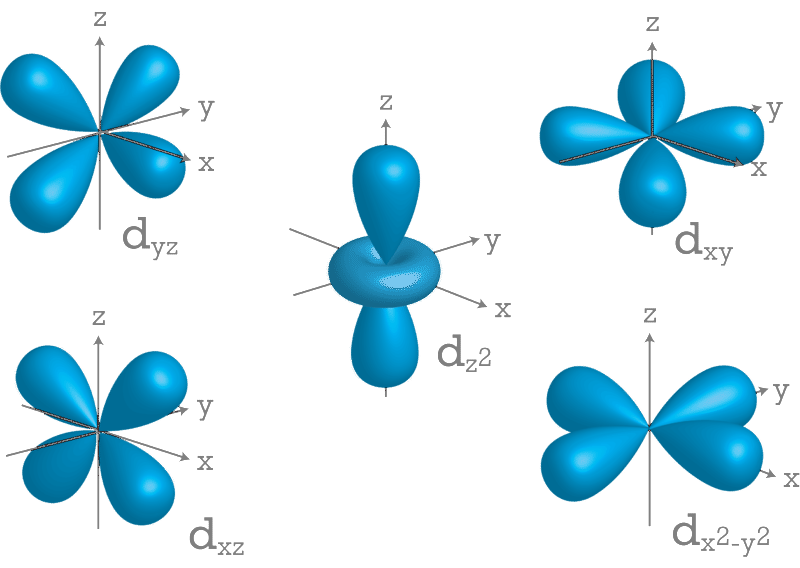
\includegraphics[width=\textwidth]{orbitais atomicos/d2}

\end{tcolorbox}

\subsection{f}
\label{oa f}

\end{multicols}

\section{Teoria dos Orbitais Moleculares TOM}
\label{tom}

\begin{multicols}{2}

	\paragraph{HOMO:} \hspace{-2mm}%
	\textbf{H}ighest
	\textbf{O}ccupied
	\textbf{M}olecular
	\textbf{O}rbital%
%
\\	\paragraph{LUMO:} \hspace{-2mm}%
	\textbf{L}owest
	\textbf{U}noccupied
	\textbf{M}olecular
	\textbf{O}rbital%

\end{multicols}


\section{Character Tables}
%
São tabelas que descrevem as características de orbitais sobre um eixo referencial
%
%A character table is a 2 dimensional chart associated with a point group that contains the irreducible representations of each point group along with their corresponding matrix characters. It also contains the Mulliken symbols used to describe the dimensions of the irreducible representations, and the functions for symmetry symbols for the Cartesian coordinates as well as rotations about the Cartesian coordinates.


{
\setlength\tabcolsep{3mm}
\renewcommand\arraystretch{2.5}

\begin{table}[H]\centering
\resizebox{\textwidth}{!}{
\begin{tabular}{ c | c | c | c }
	
	\hline
	
	\hyperref[character tables grupo de pontos]
	{
		{
		\renewcommand\arraystretch{1}
		\begin{tabular}{c}
			Grupo de
		\\	Pontos
		\end{tabular}
		}
	}
	& \multicolumn{1}{c |}
	{
		\hyperref[character tables operacoes de rotacao]
			{Operações de Rotação}
	}
	& \multicolumn{2}{c}
	{	
		\hyperref[character tables funcoes de simetria]
			{Funções de Simetria}
	}
		
	\\[1mm] \hline
	
	\hyperref[character tables mulliken]
	{
		{
		\renewcommand\arraystretch{1}
		\begin{tabular}{c}
			Símbolos de
		\\	Mulliken
		\end{tabular}
		}
	}
	& \hyperref[character tables representacao irredutivel mulliken]
		{Representação irredutível}
	& \hyperref[character tables coordenadas cartesianas e rotacao]
	{
		{
		\renewcommand\arraystretch{1}
		\begin{tabular}{c}
	  		Coordenadas Cartesianas
	  	\\	e rotações
	 	\end{tabular}
		}
	}
	& \hyperref[character tables produtos binarios e quadraticos]
	{	
		{
		\renewcommand\arraystretch{1}
		\begin{tabular}{c}
	  		Produtos binários
	  	\\	e quadraticos
		\end{tabular}
		}
	}
	
	\\[1mm] \hline

\end{tabular}
}
\end{table}
}

\subsection{Grupo de Pontos}
\label{character tables grupo de pontos}



\subsection{Operações de Rotação}
\label{character tables operacoes de rotacao}

\subsection{Símbolos de Mulliken}
\label{character tables mulliken}


{
\setlength\tabcolsep{3mm}
\renewcommand\arraystretch{1.5}

\begin{table}[H]\centering
\resizebox{.7\textwidth}{!}{
\begin{tabular}{*{2}{c}}
	
	\toprule

	{
	\renewcommand\arraystretch{1}
	\begin{tabular}{c}
		Degeneração
	\\	ou Dimensões
	\\[2mm]	
		Simbolo
		
	\end{tabular}
	}
	
	&
	{\large
	\begin{tabular}{*{6}{c}}
		1 & 1 & 2 & 3 & 4 & 5
	\\[2mm]
		A & B & E & T & G & H
		
	\end{tabular}
	}
	
	\\ \bottomrule

\end{tabular}
}
\caption{Simbolos de Mulliken por Dimensões}
\end{table}
}

\subsubsection{Subscritos do Simbolo de Mulliken}

\paragraph{1:} Simétrico com respeito ao eixo C$_n$ ou caso 
			sem eixo perpendicular, Simétrico com respeito 
			a \chemsigma\textsubscript{v}

\paragraph{2:} Anti-simétrico com respeito ao eixo C$_n$
			ou caso sem eixo perpendicular,
			Anti-simétrico com respeito a 
			\chemsigma\textsubscript{v}
		
\begin{multicols}{2}
			
\paragraph{g:} Simétrico com respeito ao invérso
\paragraph{u:} Anti-simétrico com respeito ao invérso

\vfill

\paragraph{primo:}	Simétrico com respeito a 
				\chemsigma\textsubscript{h}

\paragraph{primo duplo:} Anti-simétrico com respeito a
					\chemsigma\textsubscript{h}

\end{multicols}

\subsection{Representação irredutível dos símbolos de Mulliken}
\label{character tables representacao irredutivel mulliken}

\subsection*{Funções de simetria}
\label{character tables funcoes de simetria}

\subsection{Coordenadas Cartesianas e Rotação}
\label{character tables coordenadas cartesianas e rotacao}

\subsection{Produtos binários e quadráticos}
\label{character tables produtos binarios e quadraticos}

\section{Termodinâmica}
\label{termodinamica}



\newpage



\part{Química de Coordenação}
\label{quimica de coordenacao}
%
A química se divide em dois ramos, química orgânica e inorgânica.\\
Química inorgânica compreendem todos os compostos que não possuem ligações de carbono do tipo \ch{C-H}
%

\paragraph{Complexo de Coordenação}
\label{complexo de coordenacao}
%
São produtos de
\hyperref[Background - lewis]{reações acido-base de Lewis}
composto de 
\hyperref[elemento central]{elementos centrais}
e
\hyperref[ligandos]{ligandos}
ligados por
\hyperref[Background - ligacoes covalentes coordenadas]
	    {ligações covalentes coordenadas}.
%
\paragraph{Quesito para ser considerado um complexo de coordenação}
\begin{center}\large
\hyperref[indice de coordenacao]{índice de coordenação} > \hyperref[estado de oxidacao]{estado de oxidação}
\end{center}
%
\paragraph{Classificação}\phantom{\,}
\begin{multicols}{2}

\paragraph{Adultos:} Carga elétrica nula
\paragraph{Complexo Iônico:} Carga elétrica não nula

\end{multicols}
%

\newpage

\section{Elemento Central}
\label{elemento central}
%
Elemento metálico posicionado no centro da \hyperref[esfera de coordenacao]{esfera de coordenação},
Considerado um \hyperref[Background - lewis]{ácido de Lewis}, podendo haver mais de um como em \hyperref[complexo polinuclear]{complexos polinucleares}.
%

\subsection{Estados de Oxidação}
\label{estado de oxidacao}

{
\setlength{\tabcolsep}{4.5mm}		% Width
\renewcommand\arraystretch{.9}	% Height

\begin{table}[H]\centering
\resizebox{\textwidth}{!}{
\begin{tabular}{*{10}{c}}
	
	d1 & d2 & d3 & d4 & d5 & d6 & d7 & d8 & d9 & d10
	
	\\ \toprule
	
	Sc	
	& Ti
	& V	
	& Cr	
	& Mn	
	& Fe	
	& Co	
	& Ni	
	& Cu	
	& Zn
	
	\\ \midrule
	
	& 0	
	& 0	
	& 0	
	& 0	
	& 0	
	& 0	
	& 0	
	& [0]
	&
	
	\\
	
	& 
	& 1	
	& 1	
	& 1	
	& 1	
	& 1	
	& 1	
	& {\color{Emph}1} 
	& [1]
	
	\\
	
	& 2
	& 2
	& {\color{Emph}2}	
	& {\color{Emph}2}		
	& {\color{Emph}2}	
	& {\color{Emph}2}	
	& {\color{Emph}2}		
	& {\color{Emph}2}	 
	& {\color{Emph}2}
	
	\\
	
	{\color{Emph}3}
	& 3
	& {\color{Emph}3}	
	& {\color{Emph}3}		
	& 3	
	& {\color{Emph}3}	
	& {\color{Emph}3}		
	& 3	 
	& 3
	&
	
	\\
	
	
	& {\color{Emph}4}
	& {\color{Emph}4}
	& 4		
	& 4
	& 4	
	& 4		
	& 4	 
	& [4]
	&
	
	\\
	
	
	& 
	& {\color{Emph}5}
	& 5	
	& 5
	& 
	& 		
	& 	 
	& 
	&
	
	\\
	
	& 
	& 
	& {\color{Emph}6}	
	& 6
	& 6
	& 		
	& 	 
	& 
	&
	
	\\
	
	& 
	& 
	& 	
	& 7
	& 
	& 		
	& 	 
	& 
	&
	
	\\ \midrule
	
	Y
	& Zr
	& Nb	
	& Mo	
	& Tc	
	& Ru	
	& Rh	
	& Pd	
	& Ag	
	& Cd
	
	\\ \midrule
	
	& 
	& 	
	& 0
	& 0	
	& 0	
	& 0	
	& 0	
	& 
	&
	
	\\
	
	& 
	& 
	& 
	& 1	
	& 
	& 1	
	& 
	& {\color{Emph}1} 
	& [1]
	
	\\
	
	& 2
	& 2
	& 2	
	& [2]		
	& 2
	& 2	
	& {\color{Emph}2}		
	& 2	 
	& {\color{Emph}2}
	
	\\
	
	{\color{Emph}3}
	& 3
	& 3	
	& 3		
	& 3	
	& {\color{Emph}3}	
	& {\color{Emph}3}		
	& 	 
	& 3
	&
	
	\\
	
	
	& {\color{Emph}4}
	& 4	
	& 4
	& {\color{Emph}4}
	& 4		
	& 4	 
	& 4
	&
	&
	
	\\
	
	
	& 
	& {\color{Emph}5}
	& 5	
	& 5
	& 5
	& 5		
	& 	 
	& 
	&
	
	\\
	
	& 
	& 
	& {\color{Emph}6}	
	& 6
	& 6
	& 6	
	& 	 
	& 
	&
	
	\\
	
	& 
	& 
	& 	
	& {\color{Emph}7}
	& 7
	& 		
	& 	 
	& 
	&
	
	\\
	
	& 
	& 
	& 	
	& 
	& 8
	& 		
	& 	 
	& 
	&
	
	\\ \midrule
	
	La
	& Hf
	& Ta	
	& W	
	& Re	
	& Os
	& Ir	
	& Pt	
	& Au	
	& Hg
	
	\\ \midrule
	
	& 
	& 	
	& 0
	& 0	
	& 0	
	& 0	
	& 0	
	& [0]
	&
	
	\\
	
	& 
	& 
	& 
	& 1	
	& 
	& 1	
	& 
	& 1 
	& {\color{Emph}1} 
	
	\\
	
	& 2
	& 2
	& 2	
	& 2		
	& 2
	& 2	
	& {\color{Emph}2}		
	& [2]
	& {\color{Emph}2}
	
	\\
	
	{\color{Emph}3}
	& 3
	& 3	
	& 3		
	& {\color{Emph}3}
	& 3	
	& {\color{Emph}3}		
	& 	 
	& {\color{Emph}3}
	&
	
	\\
	
	
	& {\color{Emph}4}
	& 4	
	& {\color{Emph}4}
	& {\color{Emph}4}
	& {\color{Emph}4}	
	& {\color{Emph}4}	 
	& {\color{Emph}4}
	&
	&
	
	\\
	
	
	& 
	& {\color{Emph}5}
	& {\color{Emph}5}
	& {\color{Emph}5}
	& 5
	& 5		
	& 5 
	& 5
	& 
	
	\\
	
	& 
	& 
	& {\color{Emph}6}	
	& {\color{Emph}6}
	& 6
	& 6	
	& 6	 
	& 
	&
	
	\\
	
	& 
	& 
	& 	
	& {\color{Emph}7}
	& 7
	& 		
	& 	 
	& 
	&
	
	\\
	
	& 
	& 
	& 	
	& 
	& 8
	& 		
	& 	 
	& 
	&
	
	\\ \bottomrule

\end{tabular}
}
\caption{Estado de oxidação estáveis dos metais de transição}
\end{table}
}


\subsection{Complexos Polinucleares}
\label{complexos polinucleares}
Complexos que possuem mais de um \hyperref[elemento central]{elemento central}

\newpage

\section{Ligando}
\label{ligando}
%
Elementos diretamente ligados ao \hyperref[elemento central]{elemento central},
considerados \hyperref[Background - lewis]{bases de Lewis}
%
\begin{multicols}{2}
\textbf{Aniônicos:} Possuem carga negativa.\\
\textbf{Catiônicos:} Possuem carga positiva.
\end{multicols}
\begin{center}
\textbf{Moleculares:} Possuem carga nula.
\end{center}

\subsection{Dentação}
\label{dentacao}
%
\begin{multicols}{2}
\textbf{Monodentados:} Maximo 1 ligação\\
\textbf{Polidentados:} Mais de 1 ligação
\end{multicols}
\begin{center}
\textbf{Ambidentados:} Mais de 1 ligação mas so faz n(<max) por vez
\end{center}
%


% Exemplos dentação
%\begin{table}[H]\centering

{
\setlength{\tabcolsep}{5mm}
\renewcommand\arraystretch{1.12}
\begin{longtable}{c l c l}
	
	\multicolumn{4}{l}{\textbf{Dentação}}
	
	\\
	
	\multicolumn{1}{c}{ch}
	& \multicolumn{1}{c}{Ligando}
	& \begin{tabular}{c}
	  	Atomo
	  \\	Doador
	  \end{tabular}	
	& \multicolumn{1}{c}{Info}
	
	\\* \toprule
	
	\endhead
	
%	\\ \bottomrule
%	
%	\endfoot
	
	\\ \bottomrule \caption{Ligandos por Dentação}
	
	\endlastfoot
	
	% Monodentados
	
	\multicolumn{4}{l}{\textbf{Monodentado}}
	
	\\ \midrule
	
	   \ch{I^-} & Iodo & I
	\\ \ch{Br^-} & Bromo & Br
	\\ \ch{CH2^-} & Amido & C
	\\ \ch{OH^-} & Hidroxo & O
	\\ \ch{O^2-} & oxo & O
	\\ \ch{O2^2-} & Peroxo & O
	\\ \ch{NO3^-} & Nitrato & O
	\\ \ch{ClO4-} & Perclorato & O
	\\ \ch{N3^-} & Azido & N & Toxico
	\\ \ch{F^-} & Fluoro & F
	\\ \ch{H2O} & Aqua & O
	\\ \ch{CH3CN} & Acetonitrilo & N
	\\ py & Piridina & N
	\\ \ch{NH3} & Amin / Amino & N
	\\ \ch{PR_{n}H_{3-n}} & \hyperref[organofosfinas]{Organofosfinas} & P
	\\ \ch{CO} & Carbonil & C
	\\ \ch{CO2} & Carboxalato & C
	\\ \ch{R-C=C-R} & Alquenos & \ch{=}
	\\ \ch{Cp-} & Ciclopentadienil & \ch{=} 
	   & \begin{tabular}{@{}l@{}}
			Se liga pelo
		\\	orbital molecular
		\end{tabular}
	\\ tu & tioureio & N ou S
	
	\\ \midrule
	
	% Polidentados
	
	\multicolumn{4}{l}{\textbf{Bidentado}}
	
	\\ \midrule
	
	   \ch{C2O4^2-} & Oxalato & $2*\ch{O}$
	\\ en & Etilendiamin & $2*\ch{N}$
	\\ bipy & Bipiridil & $2*\ch{N}$
	\\ phen & fenantrolin & $2*\ch{N}$
	\\ acac & Acetilacetonato & $2*\ch{C}$
	   & \begin{tabular}{@{}l@{}}
			Tambem pode ser
		\\	Monodentado
		\\	pelo C Central
		\end{tabular}
	\\ dppe & Bis(difenilfosfin)etano 
	   & $2*\ch{P}$ & Ocupa muito espaço
	\\ \ch{dmg} & Dimetilglioxin & $2*\ch{N}$
	   & quelato(4) em pares
	
	\\ \midrule
	
	\multicolumn{4}{l}{\textbf{Tridentado}}
	
	\\ \midrule
	
	   dien & Dietilentriamin & $3*\ch{N}$
	\\ terpy & Terpiridin & $3*\ch{N}$
	   & Ocupa muito espaço
	\\ tacn & Triazaciclononano & $3*\ch{N}$
	   & Quelato(3)
	   
	\\ \midrule
	
	\multicolumn{4}{l}{\textbf{Tetradentado}}
	
	\\ \midrule
	
	   trien & Trietilentetramin & $4*\ch{N}$
	   & Quelato(3)
	\\ tren & Tris(2-aminetil)amin & $4*\ch{N}$
	   & Quelato(3)
	
	\\ \midrule
	
	\multicolumn{4}{l}{\textbf{Hexadentado}}
	
	\\ \midrule
	
	   penten & pentaetilenohexamin & $6*\ch{N}$
	   & Quelato(5)
	
	\\ \midrule
	
	% Ambidentados
	
%	\multirow{2}{*}{
%     \begin{tabular}[c]{@{\hspace{-1mm}} l @{}}
%     	Monodentado
%	\\	Ambidentado
%     \end{tabular}
%	}
	
	\multicolumn{4}{l}{\textbf{Monodentado Ambidentado}}
	
	\\ \midrule
	
	   \ch{CN^-} & Ciano & C ou N
	\\ \ch{SCN-} & Tiocianato & S
	\\ \ch{NCS-} & Isotiocianato & N
	\\ \ch{S^2-} & Tio & S
	   & Bidentado em 
	     \hyperref[complexos polinucleares]{Pontes}
	\\ \ch{Cl^-} & Cloro & Cl 
	   & Bidentado em 
	     \hyperref[complexos polinucleares]{Pontes}
	\\ \ch{OH^-} & Hidroxo & O
	   & Bidentado em 
	     \hyperref[complexos polinucleares]{Pontes}
	\\ \ch{NO2^-} & Nitro & N
	\\ \ch{ONO^-} & Nitrito & O
	\\ dppm & Bis(difenilfosfin)metano 
	   & P & Ocupa muito espaço
	\\ \ch{R-NO} & Nitroso & N ou O
	\\ \ch{CO3^{2-}} & Carbonato & O
	\\ \ch{SO3^{2-}} & Sulfito & S ou O 
	\\ \ch{SO4^{2-}} & Sulfato & O
	\\ \ch{PO4^{3-}} & Fosfato & O
	
	\\ \midrule
	
	\multicolumn{4}{l}{\textbf{Outros}}
	
	\\ \midrule
	
	   & \hyperref[crown eters]{Crown eters}
	\\ & \hyperref[corroles]{Corroles}
	\\ & \hyperref[acidos aminopolicarboxilicos]
			   {Acidos Aminopolicarboxilicos}
	\\ & \hyperref[criptandos]{Criptandos}
	\\ \ch{C4H4N2} & Pirazin & \ch{=} & ditopico
	
\end{longtable}
}

\subsection{Quelação}
\label{quelacao}
%
Numero de Anéis que um \hyperref[ligando]{ligando} faz com o \hyperref[elemento central]{elemento central}, geralmente diretamente relacionado com o numero de átomos doadores do ligando.
%

\setlength{\tabcolsep}{4mm}

{
%\setlength{\tabcolsep}{4mm}
\renewcommand\arraystretch{1.15}
\begin{table}[H]\centering
\resizebox{\textwidth}{!}{
\begin{tabular}{c c l r @{\,+\,} l c}
	
	\multicolumn{6}{l}{\textbf{Grupo}}
	
	\\
	
	\multicolumn{1}{c}{Quelação}
	& \multicolumn{1}{c}{ch}
	& \multicolumn{1}{c}{Nome}
	& \multicolumn{2}{c}{
	  \begin{tabular}{c}
	  	Átomos
	  \\ Doadores
	  \end{tabular}
	  }
	& \multicolumn{1}{c}{
	  \begin{tabular}{c}
	  	Max
	  \\ Lig
	  \end{tabular}
	  }
	
	\\ \toprule
	
	% Sem Grupo     
	
	   1 & \ch{C2O4^{2-}} & Oxalato
	     & \multicolumn{2}{c}{$2*\ch{O}$} & 4
	     
	\\ 1 & en & Etilendiamin 
	     & \multicolumn{2}{c}{$2*\ch{N}$} & 2
	     
	\\ 1 & bipy & Bipiridil 
	     & \multicolumn{2}{c}{$2*\ch{N}$} & 2
	     
	\\ 1 & fen & Fenantrolin
		& \multicolumn{2}{c}{$2*\ch{N}$} & 2
	
	\\ 1 & acac & Acetilacetonato
		& \multicolumn{2}{c}{$2*\ch{N}$} & 3
		
	\\ 1 & ddpe & Bis(difenilfosfin)etano
		& \multicolumn{2}{c}{$2*\ch{N}$} & 2
		
	\\ 2 & dien & Dietilentriamin
		& \multicolumn{2}{c}{$3*\ch{N}$} & 3
		
	\\ 2 & terpy & Terpiridin 
		& \multicolumn{2}{c}{$3*\ch{N}$} & 3
	
	\\ 3 & tacn & Triazaciclononano
		& \multicolumn{2}{c}{$3*\ch{N}$} & 3
	
	\\ 3 & trien & Trietilentetramin
		& \multicolumn{2}{c}{$4*\ch{N}$} & 4
	
	\\ 3 & tren & Tris(2-aminetil)amin
		& \multicolumn{2}{c}{$4*\ch{N}$} & 4
	
	\\ 4 & \ch{dmg2^{2-}} & Bisdimetilglioxin
		& \multicolumn{2}{c}{$4*\ch{N}$} & 4
	
	\\ 5 & penten & pentaetilenohexamin
		& \multicolumn{2}{c}{$6*\ch{N}$} & 6
	
	
	
	\\ \midrule
	
	% Acidos Aminopolicarboxilicos
	
	\multicolumn{6}{l}%
	{\textbf{Acidos Aminopolicarboxilicos}}
	
	\\ \midrule
	
	   1 & gly$^{1-}$ & glicinato 
	     & \ch{N} & \ch{O} & 2
	   
	\\ 2 & IDA$^{2-}$ & Iminodiacetato 
	     & \ch{N} & $2*\ch{O}$ & 3
	   
	\\ 3 & NTA$^{3-}$ & Nitrilotriacetato 
	     & \ch{N} & $3*\ch{O}$ & 4
		
	\\ 3 & ?$^{3-}$ & Nicotianamin
	     & $2*\ch{N}$ & $3*\ch{O}$ & 5?
		
	\\ 3 & EDDHA$^{4-}$ &
	     & $2*\ch{N}$ & $4*\ch{O}$ & 6
		
	\\ 3 & EDDS$^{4-}$ &
	     & $2*\ch{N}$ & $4*\ch{O}$ & 6
	   
	\\ 5 & DTPA$^{4-}$ & Dietilenotriaminpentacetato
	     & $3*\ch{N}$ & $5*\ch{O}$ & 8
	   
	\\ 5 & BAPTA$^{4-}$ & 
	     & $2*\ch{N}$ & $4*\ch{O}$ & 6
	   
	\\ 5 & EDTA$^{4-}$ & Etilendiamintetracetato
	     & $2*\ch{N}$ & $4*\ch{O}$ & 6
	   
	\\ 5 & EGTA$^{4-}$ & Trietilenoglicodiamintetracetico
	     & $2*\ch{N}$ & $4*\ch{O}$ & 6
	   
	\\ 6 & NOTA$^{3-}$ &
	     & $3*\ch{N}$ & $3*\ch{O}$ & 6
		
	\\ 8 & DOTA$^{4-}$ &
	     & $4*\ch{N}$ & $4*\ch{O}$ & 8
	
	\\ \midrule
	
	% Crown Eters
	
	\multicolumn{6}{l}{\textbf{Crown Eters}}
	
	\\ \midrule
	
	   4 
	   & \multicolumn{2}{r@{\qquad\qquad}}
	     {\ch{12 - crown - 4}}
	   & \multicolumn{1}{c@{}}{} & $4*\ch{O}$ & 4
	   
	\\ 5 
	   & \multicolumn{2}{r@{\qquad\qquad}}
	     {\ch{15 - crown - 5}}
	   & \multicolumn{1}{c@{}}{} & $5*\ch{O}$ & 5
	   
	\\ 6 
	   & \multicolumn{2}{r@{\qquad\qquad}}
	     {\ch{18 - crown - 6}}
	   & \multicolumn{1}{c@{}}{} & $6*\ch{O}$ & 6
	   
	\\ 6 
	   & \multicolumn{2}{r@{\qquad\qquad}}
	     {\ch{dibenzo - 18 - crown - 6}}
	   & \multicolumn{1}{c@{}}{} & $6*\ch{O}$ & 6
	   
	\\ 6 
	   & \multicolumn{2}{r@{\qquad\qquad}}
	     {\ch{diaza - 18 - crown - 6}}
	   & $2*\ch{N}$ & $4*\ch{O}$ & 6
	
	\\ \midrule
	
	% Criptandos
	
	\multicolumn{6}{l}{\textbf{Criptandos}}
	
	\\ \midrule
	
	9 & &  2.2.2-criptando & $ 6*\ch{O}$ & $2*\ch{N} $ & 8
	
	\\ \bottomrule

\end{tabular}
} \caption{Ligandos por grupo e Quelação}
\end{table}
}


\subsection{Acidos Aminopolicarboxilicos (ACPAs)}
\label{acidos aminopolicarboxilicos}

%{
%\setlength{\tabcolsep}{4mm}
\begin{table}[H]\centering
%\resizebox{\textwidth}{!}{
\begin{tabular}{c c l r@{\,+\,}l c}
	
	\multicolumn{1}{c}{Dentação}
	& \multicolumn{1}{c}{Sigla}
	& \multicolumn{1}{c}{Nome}
	& \multicolumn{2}{c}{
	  \begin{tabular}{@{}c@{}}
		Átomos
	  \\	Doadores
	  \end{tabular}
	  }
	& \multicolumn{1}{c}{Quelação}
	
	\\ \toprule
	
	   2 & gly$^{1-}$ & glicinato 
	   	& $\ch{N}$ & $\ch{O}$ & 1
		
	\\ 3 & IDA$^{2-}$ & Iminodiacetato 
		& $\ch{N}$ & $2*\ch{O}$ & 2
		
	\\ 4 & NTA$^{3-}$ & Nitrilotriacetato 
		& $\ch{N}$ & $3*\ch{O}$ & 3
		
	\\ 6 & EDTA$^{4-}$ & Etilendiamintetracetato
		& $2*\ch{N}$ & $4*\ch{O}$ & 5
		
	\\ 6 & EGTA$^{4-}$ & Trietilenoglicodiamintetracetico
		& $2*\ch{N}$ & $4*\ch{O}$ & 5
		
	\\ 8 & DTPA$^{4-}$ & Dietilenotriaminpentacetato
		& $3*\ch{N}$ & $5*\ch{O}$ & 5
		
	\\ 6 & BAPTA$^{4-}$ & 
		& $2*\ch{N}$ & $4*\ch{O}$ & 5
		
	\\ 6 & NOTA$^{3-}$ & 
		& $3*\ch{N}$ & $3*\ch{O}$ & 6
		
	\\ 8 & DOTA$^{4-}$ &
		& $4*\ch{N}$ & $4*\ch{O}$ & 8
		
	\\ 4?& ?$^{3-}$ & Nicotianamin 
		& $\ch{N}$ & $3*\ch{O}$ & 3
		
	\\ 6 & EDDHA$^{4-}$ &
		& $2*\ch{N}$ & $4*\ch{O}$ & 3
		
	\\ 6 & EDDS$^{4-}$ &
		& $2*\ch{N}$ & $4*\ch{O}$ & 3
	
	\\ \bottomrule
	
\end{tabular}
\caption{Acidos Aminopolicarboxilicos}
\end{table}
%}


\subsection{Crown Eters}
\label{crown eters}

%{
%\setlength{\tabcolsep}{4mm}
\begin{table}[H]\centering
%\resizebox{\textwidth}{!}{
\begin{tabular}{c r l c}
	
	\multicolumn{1}{c}{Dentação}
	& \multicolumn{1}{c}{Nome}
	& \multicolumn{1}{c}{
	  \begin{tabular}{@{}c@{}}
		Átomos
	  \\	Doadores
	  \end{tabular}
	  } 
	& \multicolumn{1}{c}{Quelação}
	
	\\ \toprule
	
	   4 & \ch{12 - crown - 4} 
	   	& $4*\ch{O}$ & 4
		
	\\ 5 & \ch{15 - crown - 5} 
		& $5*\ch{O}$ & 5
		
	\\ 6 & \ch{18 - crown - 6} 
		& $6*\ch{O}$ & 6
		
	\\ 6 & \ch{dibenzo - 18 - crown - 6} 
		& $6*\ch{O}$ & 6
		
	\\ 6 & \ch{diaza - 18 - crown - 6} 
		& $4*\ch{O}+2*\ch{N}$ & 6
		
	\\ \bottomrule
	
\end{tabular}
\caption{Crown Eters}
\end{table}
%}

\subsection{Criptandos}
\label{criptandos}

%{
%\setlength{\tabcolsep}{4mm}
\begin{table}[H]\centering
%\resizebox{\textwidth}{!}{
\begin{tabular}{c c c c}
	
	\multicolumn{1}{c}{Dentação}
	& \multicolumn{1}{c}{Nome}
	& \multicolumn{1}{c}{
	  \begin{tabular}{@{}c@{}}
		Átomos
	  \\	Doadores
	  \end{tabular}
	  } 
	& \multicolumn{1}{c}{Quelação}
	
	\\ \toprule
	
	8 & 2.2.2-criptando & $ 6*\ch{O}+2*\ch{N} $ & 9
	
	\\ \bottomrule
	
\end{tabular}
\caption{Criptandos}
\end{table}
%}


% Organofosfinas
\subsection{Organofosfinas}
\label{organofosfinas}

{
%\setlength\tabcolsep{6mm}
%\renewcommand\arraystretch{1.25}

\begin{table}[H]\centering
%\resizebox{\textwidth}{!}{
\begin{tabular}{c l l}
	
	\multicolumn{3}{l}{\textbf{Grupo}}
	
	\\
	
	\multicolumn{1}{c}{ch}
	& \multicolumn{1}{c}{Nome}
	& \multicolumn{1}{c}{info}
	
	\\ \toprule
	
	\multicolumn{3}{l}{\textbf{Primárias \ch{PRH2}}}
	
	\\ \midrule
	
	\multicolumn{3}{l}{\textbf{Secundárias \ch{PR2H}}}
	
	\\ \midrule
	
	\multicolumn{3}{l}{\textbf{Terciárias \ch{PR3}}}
	
	\\ \midrule
	
	   \ch{PPh3} & Trifenilfosfina
	   & Ocupa muito espaço
	\\ \ch{PCy3} & Tricyclohexylfosfino
	   & Ocupa muito espaço
	\\ \ch{Pet3} & Trietilfosfina
	\\ \ch{P(CH3)3} & Trimetilfosfino
	\\ \ch{P(CH2O)3} & Trimetilfosfito
	\\ \ch{P(o-tol)3} & Tris(o-tolil)fosfino
	\\ \ch{PF3} & trifluorofosforo
	
	\\ \midrule
	
	\multicolumn{3}{l}{\textbf{Ciclicas \ch{PR2H}}}
	
	\\ \bottomrule

\end{tabular}
%}
\caption{Organo fosfinas por grupo}
\end{table}
}




\section{Esfera de Coordenação}
\label{esfera de coordenacao}
%
\hyperref[elemento central]{Elemento central} e seus \hyperref[ligando]{ligandos} diretamente ligados
%


\section{Numero de Coordenação}
\label{numero de coordenacao}
%
Numero de ligações feitas pelo \hyperref[elemento central]{elemento central}\\
Util para classificar a geometria de Compostos
%

\subsection{Geometria}

%{
%\setlength{\tabcolsep}{4mm}
\begin{table}[H]\centering
%\resizebox{\textwidth}{!}{
\begin{tabular}{r l l}

	\multicolumn{1}{c}{NC}
	& \multicolumn{1}{c}{Geometria}
	& \multicolumn{1}{c}{Info}
	
	\\ \toprule
	
	   2 & Linear
	\\ 3 & Trigonal-Plana
	\\ 4 & Tetraédrica & Mais comum
	\\ 4 & Quadrangular-Plana & Metais d8
	\\ 5 & Bipiramide-Trigonal
	\\ 5 & Piramide de Base Quadrada & Depende dos Ligantes
	\\ 6 & Octáedricos & Mais comum
	\\ 6 & Prisma Trigonal &
	\\ 7 & Bipiramides Pentagonais & Metais Grandes
	\\ 7 & Prismáticas Trigonal Monoapicada & Metais Grandes
	\\ 8 & Cubo &
	\\ 9 & Prisma Trigonal Triapicado 
		& Ítrio, Latânio e Bloco f
	\\ 10& Cubo Octaédrica & Iões do bloco f
	
	\\ \bottomrule

\end{tabular}
\caption{Geometrias por \hyperref[numero de coordenacao]{NC}}
\end{table}
%}

\section{Distorção de Jahn-Teller}
\label{jahn-teller}
%%
%Iões metálicos do grupo \textcolor{Emph}{d4} e \textcolor{Emph}{d9} são muita vezes tetragonalmente distorcidos
%%

\setlength{\tabcolsep}{5mm}

\newcommand\jeantellerY{%
	\cellcolor{DGreen}{\textcolor{Green}{Y}}%
}
\newcommand\jeantellerN{%
	\cellcolor{DRed}{\textcolor{Red}{N}}%
}

{
%\setlength{\tabcolsep}{5mm}		% Width
%\renewcommand\arraystretch{1.25}	% Height

\begin{table}[H]\centering
\resizebox{\textwidth}{!}{
\begin{tabular}{*{10}{c}}

	\hyperref[]{Spin} & d1 & d2 & d3 & d4 & d5 & D6 & d7 & d8 & d9
	
	\\ \toprule
	
	Alto 
	& \cellcolor{DGreen}
	& \cellcolor{DGreen}
	& \cellcolor{DRed}
	& \cellcolor{DGreen}
	& \jeantellerN
	& \jeantellerY
	& \cellcolor{DGreen}
	& \cellcolor{DRed}
	& \cellcolor{DGreen}
	
	\\
	
	Baixo 
	& \multirow{-2}{*}{\jeantellerY}
	& \multirow{-2}{*}{\jeantellerY}
	& \multirow{-2}{*}{\jeantellerN}
	& \multirow{-2}{*}{\jeantellerY}
	& \jeantellerY
	& \jeantellerN
	& \multirow{-2}{*}{\jeantellerY}
	& \multirow{-2}{*}{\jeantellerN}
	& \multirow{-2}{*}{\jeantellerY}
	
	\\ \bottomrule

\end{tabular}
} \caption{Distorções de Jean-Teller}
\end{table}
}

\newpage

\section{Isomeria}
\label{isomeria}

% Imagens para cada isomeria

\begin{multicols}{2}

\subsection{Ionização}
\label{isomerismo de ionizacao}
%
Troca de um Ligandos Aniónicos de dentro e fora da \hyperref[esfera de coordenacao]{esfera de coordenação}
%

\begin{center}
	
	\ch{[Co(NH3)Br][SO4] (violeta) <->
\\	<-> [Co(NH3)SO4][Br]} (roxo)
	
\end{center}

\subsection{Hidratação}
\label{isomerismo de hidratacao}
%
Troca de ligando e Água de dentro e fora da \hyperref[esfera de coordenacao]{esfera de coordenação}
%

\begin{center}	

	\ch{[Cr(H2O)4Cl2]Cl . 2 H2O <->
\\	<-> [Cr(H2O)5Cl]Cl2 . H2O}
	
\end{center}

\subsection{Coordenação}
%
Troca de ligandos entre dois centros metálicos de um \hyperref[composto de coordenacao]{composto de coordenacao}
%

\begin{center}

	\ch{ [Co(NH3)6][Cr(CN)6] <-> [Co(CN)6][Cr(NH3)6] }

\end{center}

%\vfill

\subsection{Ligação}
\label{isomerismo de ligacao}
%
Complexos com ligandos ambientados, tem isômeros com as diversas combinações das diferentes formas de se ligarem
%

\begin{center} \ch{%
	[Co(NH3)4(N-CS)]^{2+} <->
\\	<-> [Co(NH3)4(S-CN)]^{2+} 
} \end{center}

\vspace{10mm}

\subsection{Polimerização}
\label{isomerismo de polimerizacao}
%
Complexos que tem a mesma formula porem peso molecular diferente
%

\begin{center}\ch{%
	[PtCl2(NH3)2] <-> [Pt(NH3)4][PtCl4] %
} \end{center}

\subsection{Geométrico}
\label{isomerismo geometrico}
%
Posição geométrica dos ligandos gerando combinações distintas do mesmo complexo.\\
Detectado pela determinação estrutural de difração de raios X de monocristal, espectroscopia de infra vermelho (IR) por auxiliar.
%
\begin{center}\bfseries

	Cis-Trans
\\	Fac-Mer	
\end{center}

\subsection{Óptico}
\label{isomerismo optico}
%
Quando a posição dos ligandos pode gerar um isômero espelhado
%
\begin{center}\bfseries
	Levógero($\Lambda$)-Destrógero($\Delta$)
\end{center}

\vfill

\end{multicols}

\section{Composto de Coordenação}
\label{composto de coordenacao}
%
Composto de elementos que inclui pelo menos um complexo de coordenação
%

%\break








\newpage



\part{Nomenclatura}
\label{nomenclatura}



\newpage

\part{Estabilidade}
\label{estabilidade}

\section*{Estudo Qualitativo}

\section{Teoria de Pearson (HS|AB)}
\label{hsab}

\begin{multicols}{2}

	\paragraph{Duros:} 
	\textcolor{Emph}{Não maleáveis}, Nuvem eletrônica não se deforma, fraca polarizabilidade
\\	\paragraph{Macios:}
	\textcolor{Emph}{Maleáveis}, Nuvem eletrônica facilmente deformável, Elevada polarizabilidade.
	

\end{multicols}

{
%\setlength{\tabcolsep}{5mm}		% Width
\renewcommand\arraystretch{1.3}	% Height

\begin{table}[H]\centering
%\resizebox{\textwidth}{!}{
\begin{tabular}{l r l}
	
	\multicolumn{1}{c}{Propriedade}
	& \multicolumn{1}{r}{Duro}
	& \multicolumn{1}{l}{Mole}
	
	\\ \toprule
	
	Raio Atómico/Iônico
	& Pequeno
	& Grande
	
	\\ Oxidação
	& Alto
	& Baixo ou Zero
	
	\\ Polarização
	& Baixa
	& Alta
	
	%\\ \hyprerref[tam]{HOMO}
	\\ HOMO
	& Baixo
	& Alto
	
	%\\ \hyprerref[tam]{LUMO}
	\\ LUMO
	& Alto
	& Baixo (> que HOMO da Base mole)
	
	\\ Afinidade
	& Lig iônica
	& Lig covalente
		
	\\ \bottomrule
	
\end{tabular}
\caption{Tendencias de Acidos/Bases Duros vs Moles}
\end{table}
}

\newcommand\HSABemphH{%
	\cellcolor{DRed}{\textcolor{Red}{H}}%
}
\newcommand\HSABemphI{%
	\cellcolor{DOrange}{\textcolor{Orange}{I}}%
}
\newcommand\HSABemphS{%
	\cellcolor{DYellow}{\textcolor{Yellow}{S}}%
}
\newcommand\HSABemphIH{%
	\cellcolor{DOrange!50!DRed}%
	{\textcolor{Orange!50!Red}{I}}%
}
\newcommand\HSABemphIS{%
	\cellcolor{DOrange!50!DYellow}%
	{\textcolor{Orange!50!Yellow}{I}}%
}


\subsection{Hidrogênio (H)}

{
%\setlength{\tabcolsep}{5mm}		% Width
%\renewcommand\arraystretch{1.25}	% Height


\begin{table}[H]\centering
%\resizebox{\textwidth}{!}{
\begin{tabular}{*{4}{c}}
	
	& 1- & 0 & 1+
	
	\\ \toprule
	
	H & \HSABemphS & \HSABemphI & \HSABemphH
	
	\\ \bottomrule

\end{tabular}
%}
\caption{Classificação do Hidrogênio por campo Hard-Soft}
\end{table}
}


\subsection{Metais Alcalinos e Alcalinos-terrosos (s)}
%\textcolor{Emph}{Duros} Sempre

{
\setlength{\tabcolsep}{9mm}		% Width
%\renewcommand\arraystretch{1.25}	% Height

\begin{table}[H]\centering
\resizebox{\textwidth}{!}{
\begin{tabular}{*{7}{c}}

	& 2 & 3 & 4 & 5 & 6 & 7
	
	\\ \toprule
	
	s1
	& Li
	& Na
	& K
	& Rb
	& Cs
	& Fr
	
	\\ \midrule
	
	0
	& \HSABemphH
	& \HSABemphH
	& \HSABemphH
	& \HSABemphH
	& \HSABemphH
	& \HSABemphH
	
	\\
	
	1+
	& \HSABemphH
	& \HSABemphH
	& \HSABemphH
	& \HSABemphH
	& \HSABemphH
	& \HSABemphH
	
	\\
	
	$\cdots$
	& \HSABemphH
	& \HSABemphH
	& \HSABemphH
	& \HSABemphH
	& \HSABemphH
	& \HSABemphH
	
	\\ \midrule
	
	s2
	& Be
	& Mg
	& Ca
	& Sr
	& Ba
	& Ra
	
	\\ \midrule
	
	0
	& \HSABemphH
	& \HSABemphH
	& \HSABemphH
	& \HSABemphH
	& \HSABemphH
	& \HSABemphH
	
	\\
	
	1+
	& \HSABemphH
	& \HSABemphH
	& \HSABemphH
	& \HSABemphH
	& \HSABemphH
	& \HSABemphH
	
	\\
	
	$\cdots$
	& \HSABemphH
	& \HSABemphH
	& \HSABemphH
	& \HSABemphH
	& \HSABemphH
	& \HSABemphH
	
	\\ \bottomrule

\end{tabular}
}\caption{Classificação dos metais alcalinos e alcalinos-terrosos por campo Hard-Soft}
\end{table}
}

\subsection{Metais de Transição (d)}

{
%\setlength{\tabcolsep}{5mm}		% Width
%\renewcommand\arraystretch{1.25}	% Height

\begin{table}[H]\centering
\resizebox{\textwidth}{!}{
\begin{tabular}{*{11}{c}}

	& d1 & d2 & d3 & d4 & d5 & d6 & d7 & d8 & d9 & d10
	
	\\ \toprule
	
	4
	& Sc
	& Ti
	& V
	& Cr
	& Mn
	& Fe
	& Co
	& Ni
	& Cu
	& Zn
	
	\\ \midrule
	
	0
	& 
	& \HSABemphH
	& \HSABemphH
	& \HSABemphH
	& \HSABemphI
	& \HSABemphI
	& \HSABemphI
	& \HSABemphI
	& \HSABemphS
	& 
	
	\\
	
	1+
	&
	& \HSABemphH
	& \HSABemphH
	& \HSABemphH
	& \HSABemphI
	& \HSABemphI
	& \HSABemphI
	& \HSABemphI
	& \HSABemphS
	& \HSABemphS
	
	\\
	
	2+
	&
	& \HSABemphH
	& \HSABemphH
	& \HSABemphH
	& \HSABemphIH
	& \HSABemphI
	& \HSABemphI
	& \HSABemphI
	& \HSABemphI
	& \HSABemphI
	
	\\
	
	3+
	& \HSABemphH
	& \HSABemphH
	& \HSABemphH
	& \HSABemphH
	& \HSABemphH
	& \HSABemphH
	& \HSABemphH
	&
	& \HSABemphI
	& \HSABemphI
	
	
	
	\\
	
	4+
	& 
	& \HSABemphH
	& \HSABemphH
	& \HSABemphH
	& \HSABemphH
	& \HSABemphH
	& \HSABemphH
	&
	&
	&
	
	\\
	
	5+
	&
	&
	& \HSABemphH
	& \HSABemphH
	& \HSABemphH
	&
	&
	&
	&
	&
	
	\\
	
	6+
	& 
	& 
	& 
	& \HSABemphH
	& \HSABemphH
	& \HSABemphH
	&
	&
	&
	&
	
	\\
	
	7+
	&
	&
	&
	&
	& \HSABemphH
	&
	&
	&
	&
	&
	
	\\ \midrule
	
	5
	& Y
	& Zr
	& Nb	
	& Mo	
	& Tc	
	& Ru	
	& Rh	
	& Pd	
	& Ag	
	& Cd
	
	\\ \midrule
	
	0
	& 
	& 
	& \HSABemphH
	& \HSABemphI
	& \HSABemphI
	& \HSABemphS
	& \HSABemphS
	& \HSABemphS
	& 
	& 
	
	\\
	
	1+
	&
	&
	& 
	&
	&
	&
	&
	&
	& \HSABemphS
	& \HSABemphS
	
	\\
	
	2+
	&
	& \HSABemphH
	& \HSABemphH
	& 
	& 
	& \HSABemphI
	& 
	& \HSABemphS
	& \HSABemphS
	& \HSABemphS
	
	\\
	
	3+
	& \HSABemphH
	& \HSABemphH
	& \HSABemphH
	& \HSABemphH
	&
	& 
	& \HSABemphI
	& 
	&
	&
	
	\\
	
	4+
	& 
	& \HSABemphH
	& \HSABemphH
	& \HSABemphH
	& \HSABemphH
	& \HSABemphH
	& \HSABemphH
	& \HSABemphH
	&
	&
	
	\\
	
	5+
	&
	&
	& \HSABemphH
	& \HSABemphH
	& \HSABemphH
	& \HSABemphH
	& \HSABemphH
	&
	&
	&
	
	\\
	
	6+
	&
	&
	&
	& \HSABemphH
	& \HSABemphH
	& \HSABemphH
	& \HSABemphH
	&
	&
	&
	
	\\
	
	7+
	&
	&
	&
	&
	& \HSABemphH
	& \HSABemphH
	&
	&
	&
	&
	
	\\
	
	8+
	&
	&
	&
	&
	&
	& \HSABemphH
	&
	&
	&
	&
	
	\\ \midrule
	
	6
	& Lu
	& Hf
	& Ta	
	& W	
	& Re	
	& Os
	& Ir	
	& Pt	
	& Au	
	& Hg
	
	\\ \midrule
	
	0
	& \HSABemphH
	& \HSABemphH
	& \HSABemphI
	& \HSABemphI
	& \HSABemphI
	& \HSABemphI
	& \HSABemphS
	& \HSABemphS
	& \HSABemphS
	& 
	
	\\
	
	1+
	&
	&
	&
	&
	&
	&
	&
	&
	& \HSABemphS
	& \HSABemphS
	
	\\
	
	2+
	&
	& \HSABemphH
	&
	&
	&
	& \HSABemphI
	&
	& \HSABemphS
	& \HSABemphS
	& \HSABemphS
	
	\\
	
	3+
	& \HSABemphH
	& \HSABemphH
	& \HSABemphH
	& \HSABemphH
	& \HSABemphH
	& \HSABemphH
	& \HSABemphIH
	& 
	& \HSABemphS
	&
	
	\\
	
	4+
	&
	& \HSABemphH
	& \HSABemphH
	& \HSABemphH
	& \HSABemphH
	& \HSABemphH
	& \HSABemphH
	& \HSABemphS
	&
	&
	
	\\
	
	5+
	&
	&
	& \HSABemphH
	& \HSABemphH
	& \HSABemphH
	& \HSABemphH
	& \HSABemphH
	&
	&
	&
	
	\\
	
	6+
	&
	&
	& 
	& \HSABemphH
	& \HSABemphH
	& \HSABemphH
	& \HSABemphH
	&
	&
	&
	
	\\
	
	7+
	&
	&
	&
	&
	& \HSABemphH
	& \HSABemphH
	&
	&
	&
	&
	
	\\
	
	8+
	&
	&
	&
	&
	&
	& \HSABemphH
	&
	&
	&
	&
	
	\\ \bottomrule

\end{tabular}
}
\caption{Classificação de Metais de transição por campo Hard-Soft}
\end{table}
}

\subsection{Lantanídeos e Actinídeos (f)}

{
\setlength{\tabcolsep}{3mm}		% Width
%\renewcommand\arraystretch{1.25}	% Height

\begin{table}[H]\centering
\resizebox{\textwidth}{!}{
\begin{tabular}{*{15}{c}}

	& f1 & f2 & f3 & f4 & f5 & f6 & f7 
	& f8 & f9 & f10 & f11 & f12 & f13 & f14
	
	\\ \toprule
	
	6
	& La
	& Ce
	& Pr
	& Nd
	& Pm
	& Sm
	& Eu
	& Gd
	& Tb
	& Dy
	& Ho
	& Er
	& Tm
	& Yb
	
	\\ \midrule
	
	0
	& \HSABemphH
	& 
	& 
	& 
	& 
	& 
	& 
	& 
	& 
	& 
	& 
	& 
	& 
	& 
	
	\\
	
	1+
	& \HSABemphH
	& 
	& 
	& 
	& 
	& 
	& 
	& 
	& 
	& 
	& 
	& 
	& 
	& 
	
	\\
	
	2+
	& \HSABemphH
	& 
	& 
	& 
	& 
	& 
	& 
	& 
	& 
	& 
	& 
	& 
	& 
	& 
	
	\\
	
	3+
	& \HSABemphH
	& \HSABemphH
	& \HSABemphH
	& \HSABemphH
	& \HSABemphH
	& \HSABemphH
	& \HSABemphH
	& \HSABemphH
	& \HSABemphH
	& \HSABemphH
	& \HSABemphH
	& \HSABemphH
	& \HSABemphH
	& \HSABemphH
	
	\\
	
	$\cdots$
	& \HSABemphH
	& \HSABemphH
	& \HSABemphH
	& \HSABemphH
	& \HSABemphH
	& \HSABemphH
	& \HSABemphH
	& \HSABemphH
	& \HSABemphH
	& \HSABemphH
	& \HSABemphH
	& \HSABemphH
	& \HSABemphH
	& \HSABemphH
	
	\\ \midrule
	
	7
	& Ac
	& Th
	& Pa
	& U
	& Np
	& Pu
	& Am
	& Cm
	& Bk
	& Cf
	& Es
	& Fm
	& Md
	& No
	
	\\ \midrule
	
	0
	& 
	& 
	& 
	& 
	& 
	& 
	& 
	& 
	& 
	& 
	& 
	& 
	& 
	& 
	
	\\
	
	1+
	& 
	& 
	& 
	& 
	& 
	& 
	& 
	& 
	& 
	& 
	& 
	& 
	& 
	& 
	
	\\
	
	2+
	& 
	& 
	& 
	& 
	& 
	& 
	& 
	& 
	& 
	& 
	& 
	& 
	& 
	& 
	
	\\
	
	3+
	& 
	& 
	& 
	& 
	& 
	& 
	& 
	& 
	& 
	& 
	& 
	& 
	& 
	& 
	
	\\
	
	4+
	& \HSABemphH
	& \HSABemphH
	& \HSABemphH
	& \HSABemphH
	& \HSABemphH
	& \HSABemphH
	& \HSABemphH
	& \HSABemphH
	& \HSABemphH
	& \HSABemphH
	& \HSABemphH
	& \HSABemphH
	& \HSABemphH
	& \HSABemphH
	
	\\
	
	$\cdots$
	& \HSABemphH
	& \HSABemphH
	& \HSABemphH
	& \HSABemphH
	& \HSABemphH
	& \HSABemphH
	& \HSABemphH
	& \HSABemphH
	& \HSABemphH
	& \HSABemphH
	& \HSABemphH
	& \HSABemphH
	& \HSABemphH
	& \HSABemphH
	
	\\ \bottomrule

\end{tabular}
} 
\caption{Classificação dos Lantanídeos e Actinídeos como ácidos pelo campo Hard-Soft}
\end{table}

\subsection{Famílias III a VII (p)}

{
\setlength{\tabcolsep}{12mm}		% Width
%\renewcommand\arraystretch{1.25}	% Height

\begin{table}[H]\centering
\resizebox{\textwidth}{!}{
\begin{tabular}{*{6}{c}}
	
	& p1 & p2 & p3 & p4 & p5
	
	\\ \toprule
	
	2
	& B
	& C
	& N
	& O
	& F
	
	\\ \midrule
	
	0
	& \HSABemphS
	& \HSABemphS
	& \HSABemphIH
	& \HSABemphH
	& \HSABemphH
	
	\\
	
	-1
	& 
	& \HSABemphS
	& \HSABemphH
	& \HSABemphH
	& \HSABemphH
	
	\\
	
	-2
	& 
	& \HSABemphS
	& \HSABemphH
	& \HSABemphH
	& \HSABemphH
	
	\\
	
	-3
	& 
	& 
	& \HSABemphH
	& \HSABemphH
	& \HSABemphH
	
	\\ \midrule
	
	3
	& Al
	& Si
	& P
	& S
	& Cl
	
	\\ \midrule
	
	0
	& \HSABemphS
	& \HSABemphS
	& \HSABemphS
	& \HSABemphIS
	& \HSABemphI
	
	\\
	
	-1
	& \HSABemphS
	& \HSABemphS
	& \HSABemphS
	& \HSABemphH
	& \HSABemphIH
	
	\\
	
	-2
	& \HSABemphS
	& \HSABemphS
	& \HSABemphS
	& \HSABemphH
	& \HSABemphH
	
	\\
	
	-3
	& \HSABemphS
	& \HSABemphS
	& \HSABemphS
	& 
	& \HSABemphH
	
	\\ \midrule
	
	4
	& Ga
	& Ge
	& As
	& Se
	& Br
	
	\\ \midrule
	
	0
	& \HSABemphS
	& \HSABemphS
	& \HSABemphS
	& \HSABemphS
	& \HSABemphS
	
	\\
	
	-1
	& \HSABemphS
	& \HSABemphS
	& \HSABemphS
	& 
	& \HSABemphI
	
	\\
	
	-2
	& \HSABemphS
	& \HSABemphS
	& \HSABemphS
	& 
	& 
	
	\\
	
	-3
	& \HSABemphS
	& \HSABemphS
	& \HSABemphS
	& 
	& \HSABemphS
	
	
	\\ \midrule
	
	5
	& In
	& Sn
	& Sb
	& Te
	& I
	
	\\ \midrule
	
	0
	& \HSABemphS
	& \HSABemphS
	& \HSABemphS
	& \HSABemphS
	& \HSABemphS
	
	\\
	
	-1
	& \HSABemphS
	& \HSABemphS
	& \HSABemphS
	& \HSABemphS
	& \HSABemphS
	
	\\
	
	-2
	& 
	& 
	& 
	& \HSABemphS
	& \HSABemphS
	
	
	\\ \midrule
	
	6
	& Tl
	& Pb
	& Bi
	& Po
	& At
	
	\\ \midrule
	
	0
	& \HSABemphS
	& \HSABemphS
	& \HSABemphS
	& \HSABemphS
	& \HSABemphS
	
	\\
	
	-1
	& \HSABemphS
	& \HSABemphS
	& \HSABemphS
	& \HSABemphS
	& \HSABemphS
	
	\\
	
	-2
	& 
	& 
	& 
	& \HSABemphS
	& \HSABemphS
	
	
	\\ \midrule
	
	7
	& Nh
	& Fl
	& Mc
	& Lv
	& Ts
	
	\\ \midrule
	
	0
	& \HSABemphS
	& \HSABemphS
	& \HSABemphS
	& \HSABemphS
	& \HSABemphS
	
	\\
	
	-1
	& \HSABemphS
	& \HSABemphS
	& \HSABemphS
	& \HSABemphS
	& \HSABemphS
		
	\\
	
	-2
	& 
	& 
	& 
	& 
	& \HSABemphS
	
	\\ \bottomrule

\end{tabular}
}
\caption{Bases das familias III a VII campo Hard-Soft}
\end{table}


%{
%\setlength{\tabcolsep}{5mm}		% Width
%\renewcommand\arraystretch{1.25}	% Height

\begin{table}[H]\centering
\resizebox{\textwidth}{!}{
\begin{tabular}{*{6}{c}}
	
	& p1 & p2 & p3 & p4 & p5
	
	\\ \toprule
	
	2
	& B
	& C
	& N
	& O
	& F
	
	
	\\ \midrule
	
	0
	& 
	& 
	& 
	& 
	& 
	
	\\
	
	+1
	& 
	& 
	& 
	& 
	& 
	
	\\
	
	+2
	& 
	& 
	& 
	& 
	& 
	
	\\
	
	+3
	& \HSABemphH
	& 
	& 
	& 
	& 
	
	\\ \midrule
	
	3
	& Al
	& Si
	& P
	& S
	& Cl
	
	
	\\ \midrule
	
	0
	& \HSABemphH
	& \HSABemphH
	& \HSABemphH
	& \HSABemphH
	& 
	
	\\
	
	+1
	& \HSABemphH
	& \HSABemphH
	& \HSABemphH
	& \HSABemphH
	& 
	
	\\
	
	+2
	& \HSABemphH
	& \HSABemphH
	& \HSABemphH
	& \HSABemphH
	& 
	
	\\
	
	+3
	& \HSABemphH
	& \HSABemphH
	& \HSABemphH
	& \HSABemphH
	& 
	
	\\ \midrule
	
	4
	& Ga
	& Ge
	& As
	& Se
	& Br
	
	\\ \midrule
	
	0
	& \HSABemphH
	& \HSABemphH
	& \HSABemphH
	& \HSABemphH
	& 
	
	\\
	
	+1
	& \HSABemphH
	& \HSABemphH
	& \HSABemphH
	& \HSABemphH
	& 
	
	\\
	
	+2
	& \HSABemphH
	& \HSABemphH
	& \HSABemphH
	& \HSABemphH
	& 
	
	\\
	
	+3
	& \HSABemphH
	& \HSABemphH
	& \HSABemphH
	& \HSABemphH
	& 
	
	\\ \midrule
	
	5
	& In
	& Sn
	& Sb
	& Te
	& I
	
	\\ \midrule
	
	0
	& \HSABemphI
	& \HSABemphH
	& \HSABemphH
	& 
	& 
	
	\\
	
	+1
	& \HSABemphH
	& \HSABemphH
	& \HSABemphH
	& \HSABemphH
	& 
	
	\\
	
	+2
	& 
	& \HSABemphI
	& 
	& 
	& 
	
	\\
	
	+3
	& \HSABemphH
	& 
	& \HSABemphI
	& 
	& 
	
	\\
	
	+4
	& \HSABemphH
	& \HSABemphH
	& 
	&
	& 
	
	
	\\ \midrule
	
	6
	& Tl
	& Pb
	& Bi
	& Po
	& At
	
	\\ \midrule
	
	0
	& \HSABemphS
	& \HSABemphI
	& \HSABemphI
	& 
	& 
		
	\\
	
	+1
	& \HSABemphS
	& \HSABemphI
	& \HSABemphI
	& 
	& 
	
	\\
	
	+2
	& \HSABemphS
	& \HSABemphIS
	& \HSABemphI
	& 
	& 
	
	\\
	
	+3
	& \HSABemphS
	& \HSABemphS
	& \HSABemphI
	& 
	& 
	
	\\ \bottomrule

\end{tabular}
}
\caption{Acidos das familias III a VI campo Hard-Soft}
\end{table}
%}

\newpage

\section{Lista de Ligandos}
Apenas para listar, melhor seguir as tabelas anteriores

\begin{multicols}{2}

\setlength\tabcolsep{5mm}

\subsection{Ácidos}
{
%\renewcommand\arraystretch{1.25}

\begin{table}[H]\centering
\resizebox{.50\textwidth}{!}{
\begin{tabular}{c l c}
	
	\multicolumn{3}{l}{\textbf{Classificação}}
	
	\\
	
	\multicolumn{1}{c}{ch}
	& \multicolumn{1}{c}{Nome / Grupo}
	& \multicolumn{1}{c}{%
		\begin{tabular}{c}
			Atomo
		\\	Doador
		\end{tabular}
	}
	
	\\ \toprule
	
	\multicolumn{3}{l}{\textcolor{Red}{\textbf{%
		Hard - A - Duro%
	}}}
	
	\\ \midrule
	
	   \ch{H+} & Hídron & H
	\\ \ch{BF3} & Borontrifluoro & B
	\\ \ch{AlCl3} & Aluminiotricloro & Al
	\\ \ch{SO3} & oxidosulfurico & S
	\\ \ch{NO2+} & Nitronio & N
	\\ \ch{CO2} & dioxido de carbono & C
	
	\\ \midrule
	
	\multicolumn{3}{l}{\textcolor{Orange}{\textbf{%
		In between%
	}}}
	
	\\ \midrule
	
	   \ch{B(CH3)3} & Trimetilborano & B
	\\ \ch{SO2} & Dioxido de enchofre & S
	
	\\ \midrule
	
	\multicolumn{3}{l}{\textcolor{Yellow}{\textbf{%
		Soft - B - Mole%
	}}}
	
	\\ \midrule
	
	   \ch{BH3}
	\\ \ch{I2}
	
	\\ \bottomrule

\end{tabular}
}
\caption{Ácidos ligandos classificados por HSAB}
\end{table}
}

\vfill

\subsection{Bases}
{
%\renewcommand\arraystretch{1.25}

\begin{table}[H]\centering
\resizebox{.50\textwidth}{!}{
\begin{tabular}{c l c}
	
	\multicolumn{3}{l}{\textbf{Classificação}}
	
	\\
	
	\multicolumn{1}{c}{ch}
	& \multicolumn{1}{c}{Nome / Grupo}
	& \multicolumn{1}{c}{%
		\begin{tabular}{c}
			Atomo
		\\	Doador
		\end{tabular}
	}
	
	\\ \toprule
	
	\multicolumn{3}{l}{\textcolor{Red}{\textbf{%
		Hard - A - Duro%
	}}}
	
	\\ \midrule
	
	   \ch{H2O} & Aqua & O
	\\ \ch{HO-} & Hidroxo & O
	\\ \ch{R - O-} & Alcóxidos & O
	\\ \ch{F-} & Fluoro & F
	\\ \ch{Cl-} & Cloro & Cl
	\\ \ch{PO4^{3-}} & Fosfato & O
	\\ \ch{SO4^{2-}} & Sulfato & O
	\\ \ch{CO3^{2-}} & Carbonato & O
	\\ \ch{R - CO2-} & Carboxilatos & O
	\\ \ch{ClO4-} & Perclorato & O
	\\ \ch{NO3-} & Nitrato & O
	\\ \ch{NH3} & Amin & N
	\\ \ch{N2 - R4} & Hidrazinos & N

	\\ \midrule
	
	\multicolumn{3}{l}{\textcolor{Orange}{\textbf{%
		In between%
	}}}
	
	\\ \midrule
	
	   \ch{py} & Piridina & N
	\\ \ch{NO2-} & Nitro & N
	
	\\ \midrule
	
	\multicolumn{3}{l}{\textcolor{Yellow}{\textbf{%
		Soft - B - Mole%
	}}}
	
	\\ \midrule
	
	   \ch{S - R2} & ? & S
	\\ \ch{R - S-} & Tiolatos & S
	\\ \ch{P - R3} & Fosfinos & P
	\\ \ch{P(CH2O)3} & Trimetilfosfito & P
		
	\\ \ch{As - R3} & ? & As
	\\ \ch{R-NC} & ? & ?
	
	\\ \ch{H-} & Hidreto & H
	\\ \ch{I-} & Iodo & I
	\\ \ch{SCN-} & Tiocianato & S
	\\ \ch{CN-} & Ciano & C ou N
	\\ \ch{CO} & Carbonil & C
	\\ \ch{C2H4} & Eteno & =
	\\ \ch{C6H6} & Benzeno & =
	
	\\ \bottomrule

\end{tabular}
}
\caption{Bases ligandos classificados por HSAB}
\end{table}
}


\end{multicols}




\section{Serie Irving-Willians}
\label{irving-willians}
%
Compara relativamente a contribuição que os metais de transição como elementos centrais trazem para a estabilidade do complexo, A comparação é feita com os metais no seu estado de oxidação 2+
\\
De forma geral a estabilidade aumenta com o raio atômico
%

{
\setlength\tabcolsep{2mm}
%\renewcommand\arraystretch{1.25}

\newcommand\irvwill[2]{%
	\cellcolor{Emph!#1!Black}{%
		\textcolor{White!#1!Emph!60!White}{\ch{#2}}%
	}%
}

%for i in {0..8}                 
%do
%        echo "10.0+1.12*$i^2" | bc -l
%done

\begin{table}[H]\centering
\resizebox{\textwidth}{!}{
\begin{tabular}{ *{12}{c} }

	\hline
	
	  \irvwill{10.00}{Ba}
	& \irvwill{11.12}{$<$\quad Sr}
	& \irvwill{14.48}{$<$\quad Ca}
	& \irvwill{20.08}{<\quad Mg}
	& \irvwill{27.92}{<\quad Mn}
	& \irvwill{38.00}{<\quad Fe}
	& \irvwill{50.32}{<\quad Co}
	& \irvwill{64.88}{<\quad Nu}
	& \irvwill{81.68}{<\quad Cu}
	& \irvwill{56.30}{>\quad Zn}
	
	
	\\ \hline

\end{tabular}
}
%\caption{A table}
\end{table}
}

\section{Efeito de Quelação}
\label{efeito de quelacao}
%
Complexos que apresentam \hyperref[quelacao]{anéis quelatos} são mais estáveis que complexos similares que não possuem anéis, esse efeito é percebido pela maior \hyperref[termodinamica]{variação entropica} da reação de formação do complexo
%



\newpage



\section*{Estudo Quantitativo}

\section{Equilíbrio de Complexos}

\begin{tcolorbox}

\begin{center}\large\bfseries

	Reagentes
	\ch{<=>[K\textsubscript{est}]}
	Produtos
	
\end{center}

\vspace{-6mm}

\begin{align*}
	\chemKappa_{\text{est}}
= 	\prod [\text{Produtos}]
/	\prod [\text{Reagentes}]
\end{align*}

\end{tcolorbox}

\vspace{2mm}

\begin{multicols}{2}

\begin{tcolorbox}

\begin{center}\large\bfseries
	
	M + L 
	\ch{<=>[\chemKappa\textsubscript{est}]}
	ML
	
\end{center}

\vspace{-6mm}

\begin{align*}
	\chemKappa_{\text{est}} 
= 	\frac{[ML]}
		{[M]\,[L]}
\end{align*}

\end{tcolorbox}

\begin{tcolorbox}

\begin{center}\large\bfseries

	M + $m$\,L
	\ch%
		{<=>%
		[\chembeta\textsubscript{ML\textsubscript{$m$}}]%
		[ou\ \chembeta\textsubscript{$m$}]
		}
	ML$_m$
	
\end{center}

\vspace{-6mm}

\begin{align*}
	\chembeta_{\ch{ML}_m}
=	\frac{[\text{ML}_m]}
		{[\text{M}]\,[\text{L}]^m}
\end{align*}

\end{tcolorbox}

\end{multicols}

\section{Constantes de estabilidade parciais}

{
%\setlength\tabcolsep{6mm}
%\renewcommand\arraystretch{1.25}

\begin{table}[H]\centering
\resizebox{.75\textwidth}{!}{
\begin{tabular}{c@{\quad}r@{\qquad}l}

	$1$
	& \ch{M + L <=> ML_{\phantom{1}}}
	& $\chemKappa_1 =\,$ [\text{ML}]/[\text{M}]\,[\text{L}]
	
	\\

	$2$
	& \ch{ML + L <=> ML2}%
	& $\chemKappa_2 =\,$ [\ch{ML2}]/[\text{ML}]\,[\text{L}]
	
	\\
	
	$\vdots$ & & $\,\vdots$
	
	\\
	
	$m$
	& \ch{ML$_{m-1}$ + L <=> ML$_m$}%
	& $K_m =\,$ [\ch{ML_m}]/[\ch{ML_{m-1}}]\,[\text{L}]
	
\end{tabular}
}
\end{table}
}

\subsection{Constante Global $\beta_m$}

\begin{align*}
	\chembeta_m 
= 	\prod\limits_{n=1}^{m} K_n
=	[\ch{ML}_m]/[\ch{M}]\,[\ch{L}]^m
& &
	\log\chembeta_m = \sum\limits_{n=1}^{m} \log K_n
\end{align*}



\paragraph{Comparação de constantes de estabilidade: }
Validas para complexos com mesmo \hyperref[numero de coordenacao]{numero de coordenação}


\newpage

\section*{Balanços Globais}

\begin{multicols}{2}

% Concentração Total [M]tot
\subsection{Concentração total \ch{[M]_{tot}}}

\begin{flalign*}
&
	\ch{[M]_{tot}}
= 	
	\sum\limits_{n=0}^{m} \ch{[ML_{$n$}]}
;\	
	\ch{[ML_{$i$}]} 
= 	
	K_{i}
\,	\ch{[ML_{$i-1$}]}
\,	\ch{[L]}
=	&\\&
=
	\ch{[M]\,[L]^{$i$}}
	\prod\limits_{n=1}^{i} K_{n}
=	
	\ch{[M]\,[L]^{$i$}}
\,	\beta_{i}
\implies	&\\&
\implies
	\ch{[M]_{tot}}
=	\ch{[M]}
+	\ch{[M]}
	\sum\limits_{i=1}^{m} \beta_i[L]^i	
%=	&\\&
%=	\ch{[M]} + \ch{[L]_{tot}} - \ch{[L]}
&
\end{flalign*}


% Concentração total [L]tot
\subsection{Concentração total \ch{[L]_{tot}}}

\begin{flalign*}
&
	\ch{[L]_{tot}}
=	\ch{[L]} + \sum\limits_{i=1}^{m} i\,\ch{[ML_{$i$}]}
;\	
	\ch{[ML_{$i$}]} 
= 	
	K_{i}
\,	\ch{[ML_{$i-1$}]}
\,	\ch{[L]}
=	&\\&
=
	\ch{[M]\,[L]^{$i$}}
	\prod\limits_{n=1}^{i} K_{n}
=	
	\ch{[M]\,[L]^{$i$}}
\,	\beta_{i}
\implies	&\\&
\implies
	\ch{[L]_{tot}}
=	\ch{[L]}
+	\ch{[M]}
	\sum\limits_{i=1}^{m}
	i\,\beta_i\,\ch{[L]}^{i}
%=	&\\&
%=	\ch{[L]} + \ch{[M]_{tot}} - \ch{[M]}
&
\end{flalign*}

\end{multicols}

\begin{align*}
%
\therefore
	\frac{ \ch{[L]_{tot}} - \ch{[L]} }
		{ \ch{[M]_{tot}} - \ch{[M]} }
=	\sum\limits_{i=1}^{m} i
=	(m+1)\,m/2
%
\end{align*}

\begin{multicols}{2}


% Fração Especifica
\section{Fração Especifica $\alpha$}

\begin{align*}
%
	\alpha_i 
=	\frac{\ch{[ML_{$i$}]}}{\ch{[M]_{tot}}}
& &
	\alpha_n
=	\beta_n\,\ch{[L]}^n\,\alpha_0
%
\end{align*}

\section{Numero médio de Ligandos $\overline{n}$}
\label{numero medio de ligandos}

\begin{align*}
%
	\overline{n}
=	\sum\limits_{i=1}^{m} i\,\alpha_i
=	\sum\limits_{i=1}^{m} 
	\frac{ i\,\ch{[ML_{$i$}]} }
		{ \ch{[M]_{tot}} }
=	\frac{ \ch{[L]_{tot}} - \ch{[L]} }
		{ \ch{[M]_{tot}} }
%
\end{align*}

\end{multicols}


% Experimentalmente
\section{Experimentalmente}
%
Em experimentos o meio utilizado é o aquoso assim as reações de formação das especies estudadas são de substituição onde aquo-complexos tem seus ligantes (\ch{H2O}) substituídos pelos ligantes desejados
%

\begin{center}\large

	\ch{M(H2O)_x^{$n$+} + $m$L^{$p$-} <=> ML_{$m$}^{$-p\,m+n$} + $x$H2O}

\end{center}

\subsection{Constantes de estabilidade experimentais}

\begin{align*}
&
	\beta_{\ch{ML_{$m$}}} 
=	\frac{\ch{[ML_{$m$}]}}
		{\ch{[M]\,[L]}}
& &
	\beta_{\ch{M(H2O)_{$x$}}}
=	\frac{\ch{[M(H2O)_{$x$}]}}
		{\ch{[M]\,[H2O]^{$x$}}}
& &
	K
=	\frac{\ch{[ML_{$m$}][H2O]^{$x$}}}
		{\ch{[M(H2O)_{$x$}][L]^{$m$}}}
=	\frac{\beta_{\ch{ML_{$m$}}}}
		{\beta_{\ch{M(H2O)_{$x$}}}}
&
\end{align*}

\newpage

\part{Teoria dos Orbitais Moleculares}
\label{orbitais moleculares}


\section{Teoria do Enlace de Valência}
\label{enlace de valencia}

\section{Origens}

\subsection{Werner - Rever}
%
Tenta descrever para parte dos elementos dois tipos de valência
%
\begin{multicols}{2}
	
	\paragraph{Valência Primaria}
	Estado de Oxidação
	\paragraph{Valência Secundária}
	Número de Coordenação
	
\end{multicols}

\section{Teoria do Campo Cristalino}
\label{campo cristalino}
%
Estuda a \textcolor{EmphLight}{repulsão} de 
\hyperref[ligando]{ligandos} e os 
\hyperref[oa d]{orbitais mais externos} do 
\hyperref[elemento central]{átomo central}, 
considerando os ligandos como 
\textcolor{EmphLight}{cargas pontuais}
%

\subsection{Divisão energética dos orbitais}

%
Na presença de ligandos os \hyperref[oa d]{orbitais d} 
do metal mais próximos do ligando se tornam 
\textcolor{EmphLight}{menos estáveis} enquanto os mais 
distantes se tornam \textcolor{EmphLight}{mais estaveis}, 
a energia necessária para um elétron orbitar em um orbital 
de menor estabilidade é maior
%
\paragraph{Nota:} A energia do sistema deve permanecer 
constante
%

% Octaédrico
\subsection*{Complexo Octaédrico}

\begin{tcolorbox}\centering


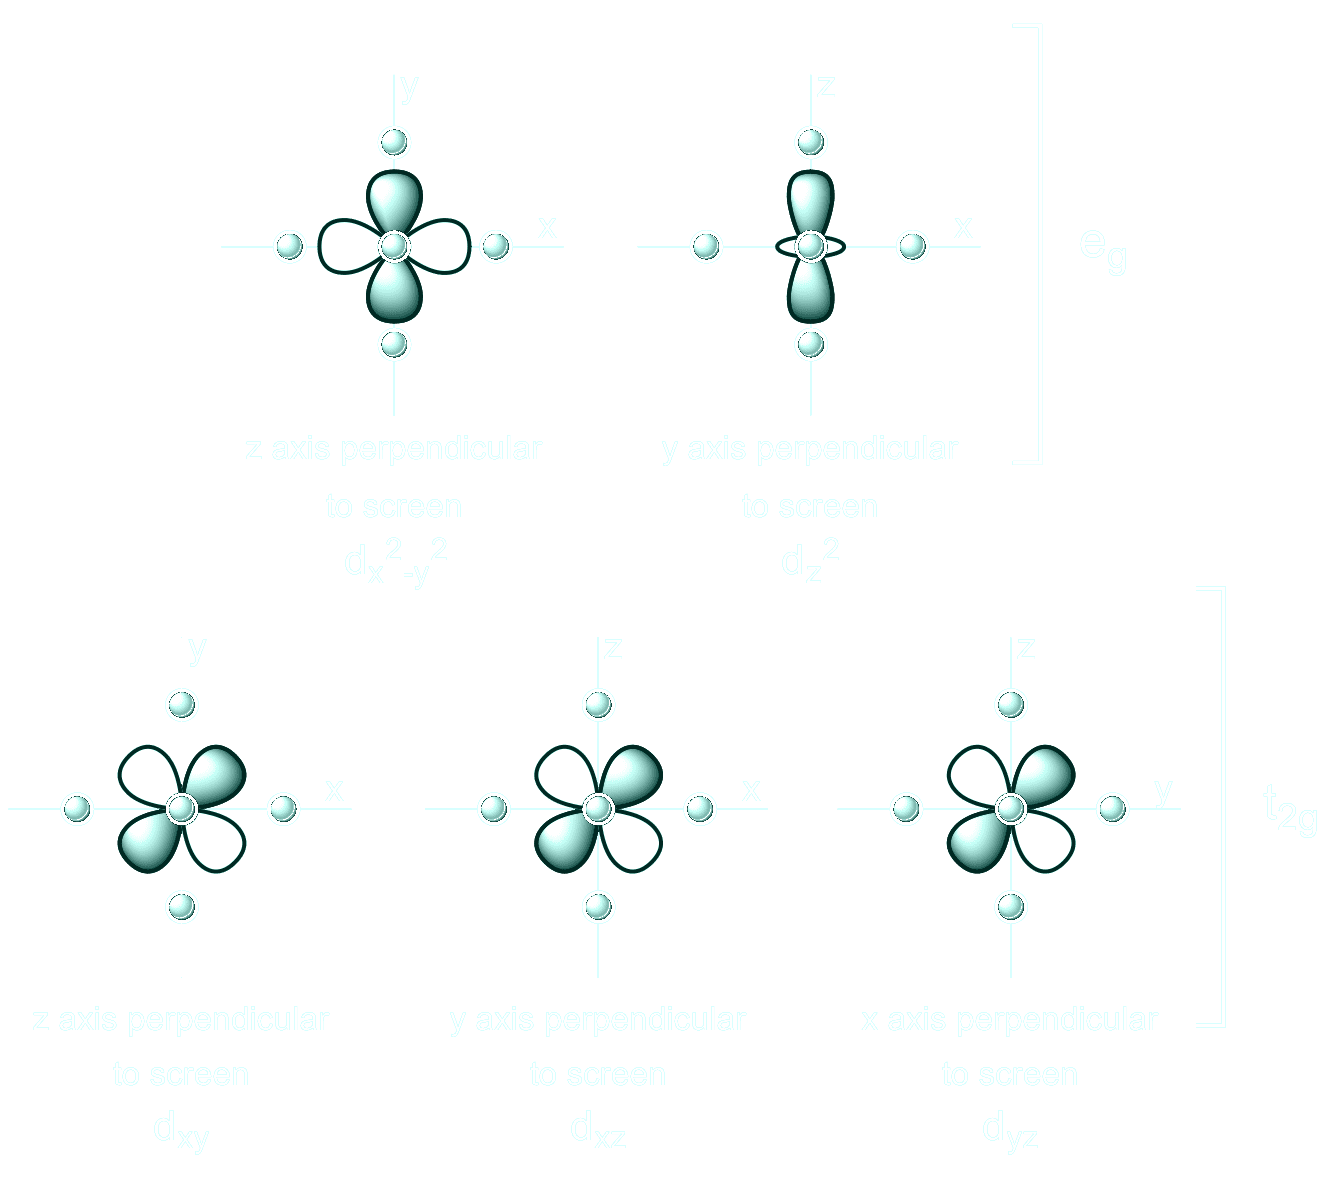
\includegraphics[width=.8\textwidth]
	{campo cristalino/octaedrico}

\resizebox{\textwidth}{!}{
\begin{modiagram}
	
	% left
	\AO(10mm){s}			{-0.10; }
	\AO(10mm){s}			{-0.05; }
	\AO[left](10mm){s}		{ 0.00; }
	\AO(10mm){s}			{ 0.05; }
	\AO(10mm){s}[label=d]	{ 0.10; }
	
	\node at (10.0mm, -1) 
	{\tiny 
		\begin{tabular}{c}
			Ausencia de 
		\\	campo exterior	
		\end{tabular}
	};
	
	% middle	
	\AO(40mm){s}			{0.90; }
	\AO(40mm){s}			{0.95; }
	\AO[middle](40mm){s}	{1.00; }
	\AO(40mm){s}			{1.05; }
	\AO(40mm){s}[label=d]	{1.10; }
	
	\node at (40mm,-1)
	{\tiny Campo Esférico};
	
	% right below
	\AO[right-below](70.0mm){s}[label=$yz$]{ .6; }
	\AO(77.5mm){s}[label=$xz$]{ .6; }
	\AO(85.0mm){s}[label=$xy$]{ .6; }
	
	% right above
	\AO[right-above]
	   (77.5mm){s}[label=$x^2$-$y^2$]	{1.6; }
	\AO(85.0mm){s}[label=$z^2$]		{1.6; }
	
	\node at (77.5mm, -1) 
	{\tiny Campo Octaédrico};
	
	\draw[<-|] 
	(65mm,1.6)
	-- node[above left]{\tiny $+0.6\,\Delta_{\text{oct}}$} 
	(65mm,1.0);
	
	\draw[->]
	(65mm,1.0)
	-- node[below left]{\tiny $-0.4\,\Delta_{\text{oct}}$}
	(65mm,0.6);
	
	\draw[<->] 
	(95mm,1.6) 
		node[left] {\tiny e\textsubscript{g}}
		node[below right]{\tiny $\Delta _{\text{oct}}$ }
	-- 
		node[above=2.5mm, right=4mm, rotate=-90]{\tiny=}
	(95mm,0.6) 
		node[left] {\tiny t\textsubscript{2g}}
		node[above right]{\tiny $10\,\text{Dq}$};
	
	\connect{
		left & middle, 
		middle & right-above, 
		middle & right-below
	}
	
	\EnergyAxis
	\node at (0,1)[above, rotate=90]{\tiny Energia};

\end{modiagram}
}



\end{tcolorbox}


% Tetraédrico
\subsection*{Complexo Tetaédrico}
\begin{tcolorbox}\centering

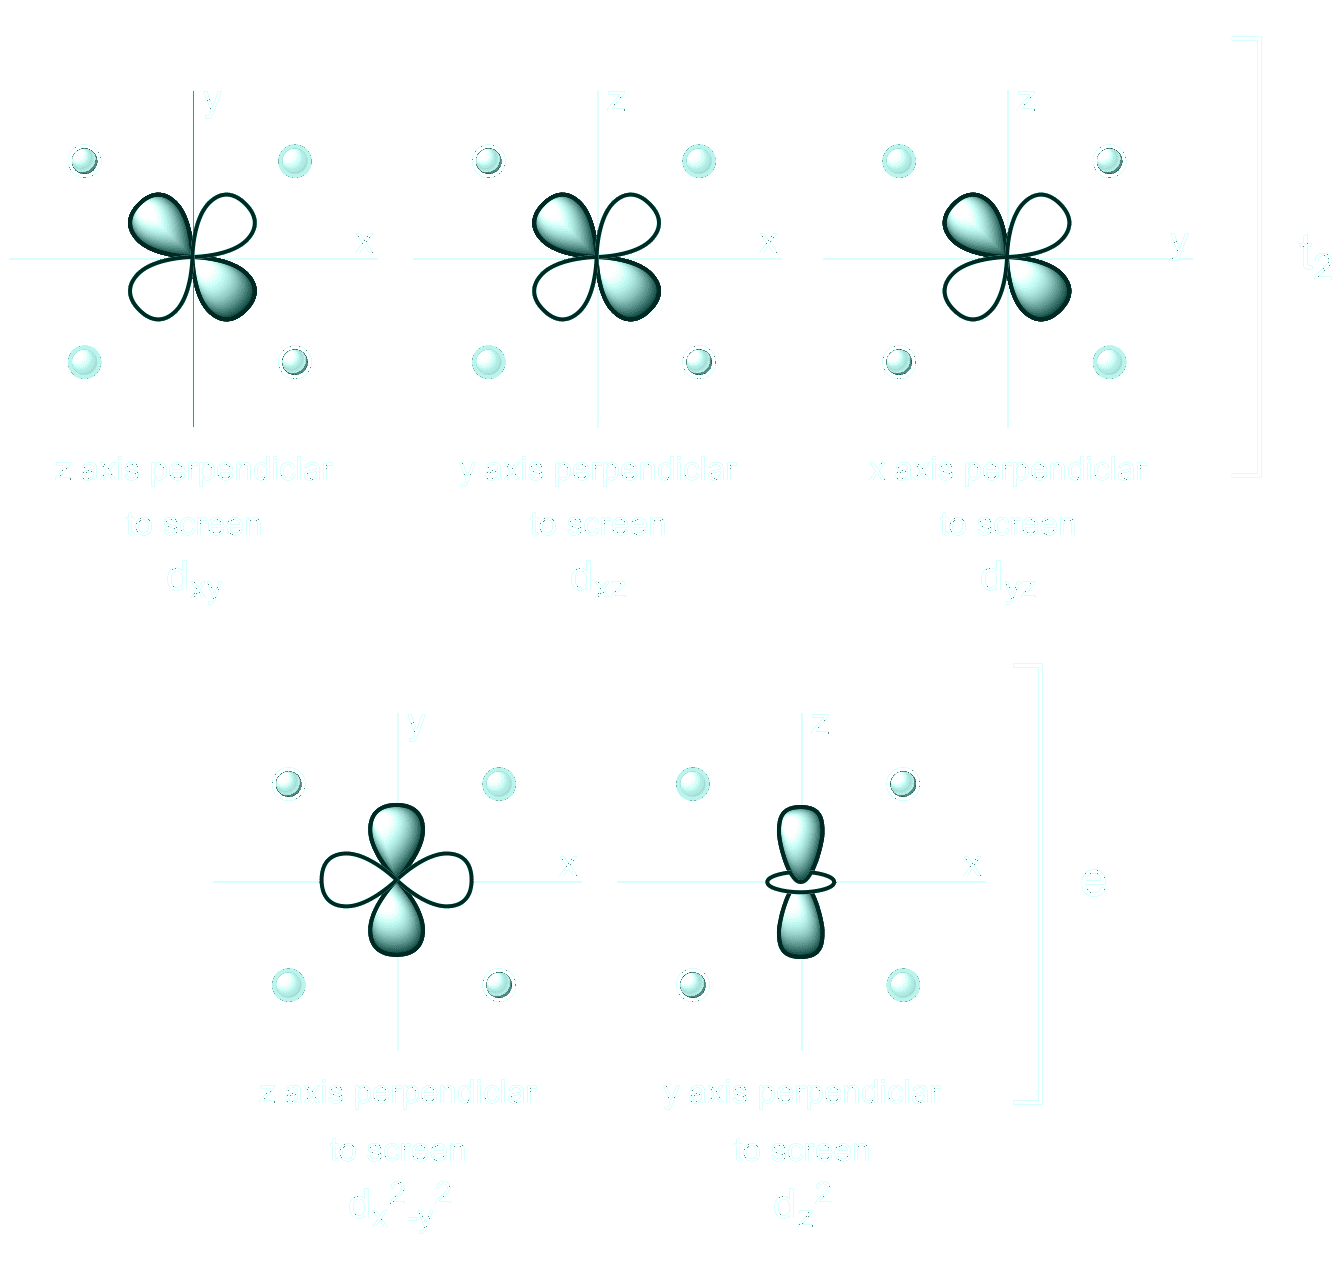
\includegraphics[width=.8\textwidth]
	{campo cristalino/tetraedrico}

\resizebox{\textwidth}{!}{
\begin{modiagram}
	
	% left
	\AO(10mm){s}			{-0.10; }
	\AO(10mm){s}			{-0.05; }
	\AO[left](10mm){s}		{ 0.00; }
	\AO(10mm){s}			{ 0.05; }
	\AO(10mm){s}[label=d]	{ 0.10; }
	
	\node at (10.0mm, -1) 
	{\tiny 
		\begin{tabular}{c}
			Ausencia de 
		\\	campo exterior	
		\end{tabular}
	};
	
	% middle	
	\AO(40mm){s}			{0.90; }
	\AO(40mm){s}			{0.95; }
	\AO[middle](40mm){s}	{1.00; }
	\AO(40mm){s}			{1.05; }
	\AO(40mm){s}[label=d]	{1.10; }
	
	\node at (40mm,-1)
	{\tiny Campo Esférico};
	
	% right above
	\AO[right-below]
	   	(70.0mm){s}[label=$yz$]{1.4; }
	\AO	(77.5mm){s}[label=$xz$]{1.4; }
	\AO	(85.0mm){s}[label=$xy$]{1.4; }
	
	% right below
	\AO[right-above]
	   (77.5mm){s}[label=$x^2$-$y^2$]	{0.4; }
	\AO(85.0mm){s}[label=$z^2$]		{0.4; }
	
	\node at (77.5mm, -1) 
	{\tiny Campo Tetraédrico};
	
	\draw[<-|] 
	(65mm,1.4)
	-- node[above left]{\tiny $+0.6\,\Delta_{\text{t}}$} 
	(65mm,1.0);
	
	\draw[->]
	(65mm,1.0)
	-- node[below left]{\tiny $-0.4\,\Delta_{\text{t}}$}
	(65mm,0.4);
	
	\draw[<->] 
	(95mm,1.4) 
		node[left] {\tiny t\textsubscript{2}}
		node[below right]{\tiny $\Delta _{\text{t}}$ }
	-- 
		node[above=2.5mm, right=3mm, rotate=-90]{\tiny=}
	(95mm,0.4) 
		node[left] {\tiny e}
		node[above right]{\tiny $10\,\text{Dq}$};
	
	\connect{
		left & middle, 
		middle & right-above, 
		middle & right-below
	}
	
	\EnergyAxis
	\node at (0,1)[above, rotate=90]{\tiny Energia};

\end{modiagram}
}

\end{tcolorbox}


\newpage


\begin{multicols}{2}

\subsection*{Campo fraco/Spin alto}
%\vspace{-5mm}

\begin{tcolorbox}\centering

\resizebox{!}{5cm}{
\begin{modiagram}
	
	% right below
	\AO[right-below]
		( 5.0mm){s}[label=$yz$]{-.4;pair}
	\AO	(12.5mm){s}[label=$xz$]{-.4;up}
	\AO	(20.0mm){s}[label=$xy$]{-.4;up}
	
	% right above
	\AO[right-above]
	   (12.5mm){s}[label=$x^2$-$y^2$]	{.6;up}
	\AO(20.0mm){s}[label=$z^2$]		{.6;up}
	
	\draw[<->] 
	(30mm,.6) node[left] {\tiny e\textsubscript{g}}
	-- node[right]
			{\tiny 
			\chemDelta\textsubscript{oct}
			$<$
			P
			}
	(30mm,-.4) node[left] {\tiny t\textsubscript{2g}};
	
	\draw[- Latex] (0,-2) -- (0,2.2);
	\node at (0,0)[above, rotate=90]{\tiny Energia};

\end{modiagram}
}

\end{tcolorbox}

%\vfill

\subsection*{Campo forte/Spin baixo}

\begin{tcolorbox}\centering

\resizebox{!}{5cm}{
\begin{modiagram}
	
	% right below
	\AO[right-below]
		( 5.0mm){s}[label=$yz$]{-1.2;pair}
	\AO	(12.5mm){s}[label=$xz$]{-1.2;pair}
	\AO	(20.0mm){s}[label=$xy$]{-1.2;pair}
	
	% right above
	\AO[right-above]
	   (12.5mm){s}[label=$x^2$-$y^2$]	{1.8;}
	\AO(20.0mm){s}[label=$z^2$]		{1.8;}
	
	\draw[<->] 
	(30mm, 1.8) node[left] {\tiny e\textsubscript{g}}
	-- node[right]
			{\tiny 
			\chemDelta\textsubscript{oct}
			$>$
			P
			}
	(30mm,-1.2) node[left] {\tiny t\textsubscript{2g}};
	
	\draw[- Latex] (0,-2) -- (0,2.2);
	\node at (0,0)[above, rotate=90]{\tiny Energia};
	
\end{modiagram}
}

\end{tcolorbox}

\end{multicols}


% talvez incluir em campo forte/fraco
\subsection{para/dia magnetismo}

\subsection{Fatores que influenciam}

%\begin{multicols}{2}
%\begin{enumerate}[left=0mm]
%	
%	\item Estado de oxidação do ion metálico
%	\item Natureza do ion  metálico
%	\item Natureza do Ligando
%	
%\end{enumerate}
%\end{multicols}

{


\setlength\tabcolsep{2mm}
%\renewcommand\arraystretch{1.25}

\newcommand\tsuchida[2]%
	{\cellcolor{Emph!#1!Black}%
		{\textcolor{White!#1!Emph!60!White}{\ch{#2}}}
	}

%for i in {0..8}                 
%do
%        echo "10.0+1.12*$i^2" | bc -l
%done

\subsubsection{Natureza do ion Metálico}
%
Diretamente proporconal:
\begin{itemize}
\item Estado de Oxidação
\item Periodo da tabela dos elementos
\end{itemize}
%

\begin{table}[H]\centering
\resizebox{\textwidth}{!}{
\begin{tabular}{ *{9}{c} }
	
	% 15 uniques
	
	\hline
	
%	\begin{tabular}{@{}*{13}{c}@{}}
	
	  \tsuchida{10.00}{				Mn^{2+}}
	& \tsuchida{11.12}{<\quad 		Ni^{2+}}
	& \tsuchida{14.48}{<\quad 		Co^{2+}}
	& \tsuchida{20.08}{<\quad 		Fe^{2+}}
	& \tsuchida{27.92}{<\quad 		V^{2+}}
	& \tsuchida{38.00}{<\quad 		Fe^{3+}}
	& \tsuchida{50.32}{<\quad 		Cr^{3+}}
	& \tsuchida{64.88}{<\quad 		V^{3+}}
	& \tsuchida{81.68}{<\quad 		Co^{3+}}
	
%	\end{tabular}
	
	\\ \hline

\end{tabular}
}
\caption{Série Espectroquímica ou Série de Tsuchida dos Metais}
\end{table}


\subsubsection{Natureza do Ligando}

\begin{table}[H]\centering
\resizebox{\textwidth}{!}{
\begin{tabular}{ *{13}{c} }
	
	% 15 uniques
	
	\hline
	
%	\begin{tabular}{@{}*{13}{c}@{}}
	
	  \tsuchida{10.000}{				I-}
	& \tsuchida{10.175}{<\quad 		Br-}
	& \tsuchida{10.700}{<\quad 		S^{2-}}
	& \tsuchida{11.575}{<\quad 		SCN-}
	& \tsuchida{11.900}{\lesssim\quad 	Cl-}
	& \tsuchida{12.800}{<\quad 		N3-}
	& \tsuchida{14.375}{<\quad 		F-}
	& \tsuchida{16.300}{<\quad 		NCO-}
	& \tsuchida{18.575}{<\quad 		OH-}
	& \tsuchida{21.200}{<\quad 		ox^{2-}}
	& \tsuchida{24.175}{<\quad 		H2O}
	& \tsuchida{27.500}{<\quad 		acac-}
	& \tsuchida{31.175}{<\quad 		NCS-}
	
%	\end{tabular}
	
	\\ \hline
	
%	\begin{tabular}{@{}*{13}{c}@{}}
	
	  \tsuchida{31.175}{				NCS-}
	& \tsuchida{35.200}{<\quad 		CH3CN}
	& \tsuchida{39.575}{<\quad 		gly}
	& \tsuchida{44.300}{<\quad 		py}
	& \tsuchida{49.375}{<\quad 		NH3}
	& \tsuchida{51.375}{\lesssim\quad 	en}
	& \tsuchida{54.800}{<\quad 		bpy}
	& \tsuchida{60.575}{<\quad 		phen}
	& \tsuchida{62.575}{\lesssim\quad 	NO2-}
	& \tsuchida{66.700}{<\quad	 	PPh3}
	& \tsuchida{66.700}{\approx\quad 	PR3}
	& \tsuchida{73.175}{<\quad 		CN-}
	& \tsuchida{77.000}{\lesssim\quad 	CO}
	
%	\end{tabular}
	
	\\ \hline

\end{tabular}
}
\caption{Série Espectroquímica ou Série de Tsuchida dos Ligandos}
\end{table}
}

\subsection{Energia de Estabilização dos Campo de Ligandos EECL}

{\large\bfseries\boldmath
\begin{align*}
	\textbf{EECL}
=	(l*0.4-h*0.6)\,\chemDelta\textsubscript{oct}
-	n*\textbf{P}
\end{align*}
}

\begin{multicols}{2}
\begin{itemize}[left=0mm]
	
	\item $h$: Elétrons no campo de maior energia
	\item $l$: Elétrons no campo de menor energia
	\item $n$: Pares eletrônicos
	
\end{itemize}
\end{multicols}

\section*{Aplicações do Campo Cristalino}

\subsection{Espectro de Frequência de Absorção de Luz}

%\section{Teoria do Campo Cristalino}
%\label{campo cristalino}
%%
%Estuda a \textcolor{EmphLight}{repulsão} de \hyperref[ligando]{ligandos} e os orbitais mais externos do \hyperref[elemento central]{átomo central}, considerando os ligandos como \textcolor{EmphLight}{cargas pontuais}
%%
%%
%
%\vspace{1mm}
%
%{
%%\setlength\tabcolsep{6mm}
%%\renewcommand\arraystretch{1.25}
%\begin{tcolorbox}
%
%	\textbf{Fatores que contribuem para a diferença energética entre orbitais}
%	\begin{itemize}[left=0mm]
%	
%		\item Natureza do \hyperref[elemento central]
%							  {elemento central}
%							  
%		\item O estado de oxidação do 
%			 \hyperref[elemento central]{elemento central}
%		\\	 Um maior \hyperref[estado de oxidacao]
%						    {estado de oxidação}
%			 leva a maiores diferenças energéticas
%			 relativas ao campo esférico
%		
%		\item O arranjo dos ligandos
%			 
%		\item O \hyperref[numero de coordenacao]
%					  {numero de coordenação}
%					  
%		\item \hyperref[serie espectroquimica]
%			 {A natureza dos ligandos}
%		
%		\item Quanto mais forte o efeito dos ligandos, 
%			 mais forte será a diferença energética dos
%			 campos.
%	
%	\end{itemize}
%
%\end{tcolorbox}
%
%\subsection{Divisão energética do orbital d metálico}
%
%\subsection*{Orbital octaédrico}
%%
%Na presença de ligandos os \hyperref[oa d]{orbitais d} do metal mais próximos do ligando se tornam \textcolor{EmphLight}{menos estáveis} enquanto os mais distantes se tornam \textcolor{EmphLight}{mais estaveis}, a energia necessária para um elétron orbitar em um orbital de menor estabilidade é maior
%%
%\paragraph{Nota:} A energia do sistema deve permanecer constante
%%
%
%\begin{center}
%
%\resizebox{\textwidth}{!}{
%\begin{modiagram}
%	
%	% left
%	\AO(10mm){s}			{-0.10; }
%	\AO(10mm){s}			{-0.05; }
%	\AO[left](10mm){s}		{ 0.00; }
%	\AO(10mm){s}			{ 0.05; }
%	\AO(10mm){s}[label=d]	{ 0.10; }
%	
%	\node at (10.0mm, -1) 
%	{\tiny 
%		\begin{tabular}{c}
%			Ausencia de 
%		\\	campo exterior	
%		\end{tabular}
%	};
%	
%	% middle	
%	\AO(40mm){s}			{0.90; }
%	\AO(40mm){s}			{0.95; }
%	\AO[middle](40mm){s}	{1.00; }
%	\AO(40mm){s}			{1.05; }
%	\AO(40mm){s}[label=d]	{1.10; }
%	
%	\node at (40mm,-1)
%	{\tiny Campo Esférico};
%	
%	% right below
%	\AO[right-below](70.0mm){s}[label=$yz$]{ .4; }
%	\AO(77.5mm){s}[label=$xz$]{ .4; }
%	\AO(85.0mm){s}[label=$xy$]{ .4; }
%	
%	% right above
%	\AO[right-above]
%	   (77.5mm){s}[label=$x^2$-$y^2$]	{1.6; }
%	\AO(85.0mm){s}[label=$z^2$]		{1.6; }
%	
%	\node at (77.5mm, -1) 
%	{\tiny Campo Octaédrico};
%	
%	\draw[<-|] 
%	(65mm,1.6)
%	-- node[above left]{\tiny $+0.6\,\Delta_{\text{oct}}$} 
%	(65mm,1.0);
%	
%	\draw[->]
%	(65mm,1.0)
%	-- node[below left]{\tiny $-0.4\,\Delta_{\text{oct}}$}
%	(65mm,0.4);
%	
%	\draw[<->] 
%	(95mm,1.6) 
%		node[left] {\tiny e\textsubscript{g}}
%		node[below right]{\tiny $\Delta _{\text{oct}}$ }
%	-- 
%		node[above=3mm, right=4mm, rotate=-90]{=}
%	(95mm,0.4) 
%		node[left] {\tiny t\textsubscript{2g}}
%		node[above right]{\tiny $10\,\text{Dq}$};
%	
%	\connect{
%		left & middle, 
%		middle & right-above, 
%		middle & right-below
%	}
%	
%	\EnergyAxis
%	\node at (0,1)[above, rotate=90]{\tiny Energia};
%
%\end{modiagram}
%}
%
%\end{center}
%
%%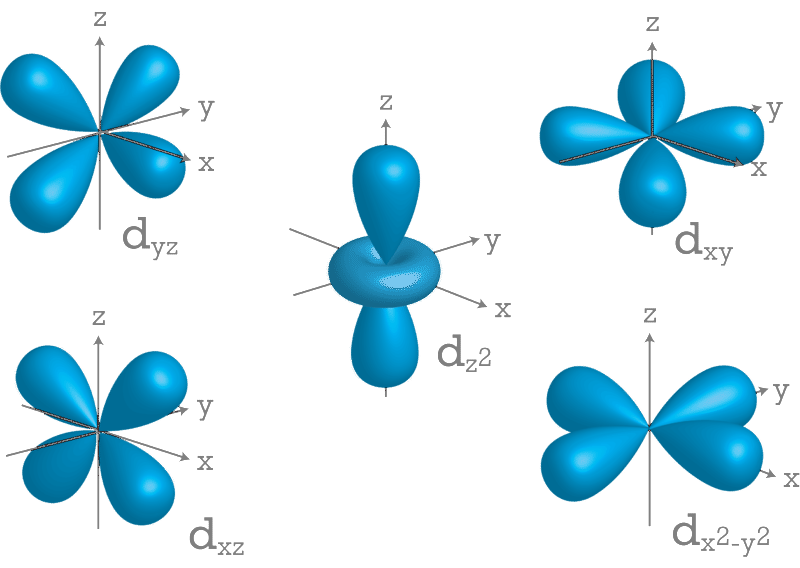
\includegraphics[width=.3\textwidth]{orbitais atomicos/d2}
%
%\newpage
%
%\subsection{Natureza dos Ligandos}
%\label{serie espectroquimica}
%
%{
%\setlength\tabcolsep{2mm}
%%\renewcommand\arraystretch{1.25}
%
%\newcommand\tsuchida[2]%
%	{\cellcolor{Emph!#1!Black}%
%		{\textcolor{White!#1!Emph!60!White}{\ch{#2}}}
%	}
%
%%for i in {0..8}                 
%%do
%%        echo "10.0+1.12*$i^2" | bc -l
%%done
%
%\begin{table}[H]\centering
%\resizebox{\textwidth}{!}{
%\begin{tabular}{ *{10}{c} }
%	
%	% 15 uniques
%	
%	\hline
%	
%	  \tsuchida{10.00}{				I-}
%	& \tsuchida{15.00}{<\quad 		Br-}
%	& \tsuchida{20.00}{<\quad 		S^{2-}}
%	& \tsuchida{25.00}{<\quad 		SCN-}
%	& \tsuchida{25.00}{\approx\quad 	Cl-}
%	& \tsuchida{30.00}{<\quad 		NO3-}
%	& \tsuchida{35.00}{<\quad 		F-}
%	& \tsuchida{40.00}{<\quad 		OH-}
%	& \tsuchida{45.00}{<\quad 		ox^{2-}}
%	& \tsuchida{50.00}{<\quad 		NCS-}
%
%	\\ \hline
%	
%	  \tsuchida{50.00}{				NCS-}
%	& \tsuchida{55.00}{<\quad 		CH3CN}
%	& \tsuchida{60.00}{<\quad 		NH3}
%	& \tsuchida{60.00}{\approx\quad 	en}
%	& \tsuchida{65.00}{<\quad 		bpy}
%	& \tsuchida{70.00}{<\quad 		phen}
%	& \tsuchida{70.00}{\approx\quad 	NO2-}
%	& \tsuchida{75.00}{<\quad 		PR3}
%	& \tsuchida{80.00}{<\quad 		CN-}
%	& \tsuchida{80.00}{\approx\quad 	CO}
%	
%	\\ \hline
%
%\end{tabular}
%}
%\caption{Série Espectroquímica ou Série de Tsuchida}
%\end{table}
%}
%
%\subsection{Energia de Estabilização de Campo de Ligandos EECL}
%\label{eecl}


\section{Teoria do Campo Ligando}
\label{campo ligando}
%
Aplicação de \hyperref[tom]{TOM} em complexos, com foco nos orbitais d
%


\newpage

\part{Reatividade}
\label{reatividade}

\end{document}








